%%%% ijcai11.tex

\typeout{IJCAI-13 Instructions for Authors}

% These are the instructions for authors for IJCAI-13.
% They are the same as the ones for IJCAI-11 with superficical wording
%   changes only.

\documentclass{article}
% The file ijcai13.sty is the style file for IJCAI-13 (same as ijcai07.sty).
\usepackage{ijcai13}

 \let\oldthebibliography=\thebibliography
  \let\endoldthebibliography=\endthebibliography
  \renewenvironment{thebibliography}[1]{%
    \begin{oldthebibliography}{#1}%
      \setlength{\parskip}{0ex}%
      \setlength{\itemsep}{1.5ex}%
  }%
  {%
    \end{oldthebibliography}%
  }

% Use the postscript times font!
\usepackage{times}
\usepackage{hyperref}

\newcommand{\note}[1]{}
% comment out the next line to turn off notes
\renewcommand{\note}[1]{~\\\frame{\begin{minipage}[c]{0.48\textwidth}\vspace{2pt}\center{#1}\vspace{2pt}\end{minipage}}\vspace{3pt}\\}

\newcommand{\hide}[1]{}


%dvips -Ppdf -tletter -G0 -o paper.ps paper.dvi

\usepackage{amsmath,amsthm,amssymb}
%\usepackage{amsfonts}

\usepackage{color}
\definecolor{Blue}{rgb}{0.9,0.3,0.3}

%http://www-db.stanford.edu/~manku/latex.html
%The itemize environment can be replaced by:
\newcommand{\squishlist}{
   \begin{list}{$\bullet$}
    { \setlength{\itemsep}{0pt}      \setlength{\parsep}{3pt}
      \setlength{\topsep}{3pt}       \setlength{\partopsep}{0pt}
      \setlength{\leftmargin}{1.5em} \setlength{\labelwidth}{1em}
      \setlength{\labelsep}{0.5em} } }

\newcommand{\squishlisttwo}{
   \begin{list}{$\bullet$}
    { \setlength{\itemsep}{0pt}    \setlength{\parsep}{0pt}
      \setlength{\topsep}{0pt}     \setlength{\partopsep}{0pt}
      \setlength{\leftmargin}{2em} \setlength{\labelwidth}{1.5em}
      \setlength{\labelsep}{0.5em} } }

\newcommand{\squishend}{
    \end{list}  }

%Example usage: \squishlist    %% \begin{itemize}
%\item First item
%\item Second item
%\squishend     %% \end{itemize}

\newcommand{\denselist}{\itemsep 0pt\topsep-6pt\partopsep-6pt}

%% a trick that makes the title take up less space for many style files (but not article)
%\addtolength{\titlebox}{-1.8cm}

%% densify spacing in bibliographies
\newcommand{\bibfix}{%    PUT \bibfix in file.bbl after first line
    \setlength{\parsep}{\parskip}%
    \setlength{\itemsep}{0cm}%
    \setlength{\topsep}{\parskip}%
    \setlength{\parskip}{0cm}%
    \setlength{\partopsep}{0cm}%
    \setlength{\listparindent}{\parindent}%
    \setlength{\labelwidth}{10pt}%
    \setlength{\labelsep}{0pt}%
    \setlength{\leftskip}{0pt}%
    \setlength{\leftmargin}{0pt}%
}

%% change margins
%\setlength{\textwidth}{7in}
%\setlength{\textheight}{8.75in}
%\setlength{\oddsidemargin}{-0.25in}
%\setlength{\evensidemargin}{-0.25in}
%\setlength{\headsep}{10pt}

%Use changebar.sty  to track changes.

%Saving space: see
%   http://www-h.eng.cam.ac.uk/help/tpl/textprocessing/squeeze.html

%Page layout info:
%   http://amath.colorado\edu/documentation/LaTeX/reference/layout.html


%%%%%%%%%% Code listings



%Latex
%\documentstyle[fleqn,psfig,epsfig]{article}
%\documentstyle[psfig]{article}
%\setlength{\textwidth}{6.5in}
%\setlength{\oddsidemargin}{0in}
%\setlength{\textheight}{8.5in}
%\setlength{\headheight}{0in}
%\setlength{\headsep}{0in}
%\setlength{\parindent}{0in} % block style
%\setlength{\parskip}{0.3cm}

\newtheorem{example}{Example}[section]
\newtheorem{thm}{Theorem}[section]
\newtheorem{cor}{Corollary}[section]
\newtheorem{defn}{Definition}[section]
\newenvironment{mythm}{{\bf Theorem}}{}
\newenvironment{myproof}{{\bf Proof}}{}

%http://www.maths.tcd.ie/~dwilkins/LaTeXPrimer/Theorems.html
%\newenvironment{proof}[1][Proof]{\begin{trivlist}
%\item[\hskip \labelsep {\bfseries #1}]}{\end{trivlist}}

% make qed symbol a solid square
%\renewcommand{\qed}{\mbox{$\hrulefill \blacksquare $}}

%http://everything2.com/title/tombstone
%\renewcommand{\qed}{\hfill \nobreak \ifvmode \relax \else
%    \ifdim\lastskip<1.5em \hskip-\lastskip
%    \hskip1.5em plus0em minus0.5em \fi \nobreak
%    \vrule height0.4em width0.4em depth0.25em\fi}


%\newcommand{\subsubsubsection}[1]{\paragraph{#1}}
\newcommand{\choice}[2]{\left(\!\!\! \begin{array}{c} #1 \\ #2\end{array} \!\!\!\right)}
%\newcommand{\half}{\frac{1}{2}}
\newcommand{\half}{\frac{1}{2}}
%\newcommand{\defeq}{\stackrel{\rm def}{=}}
\newcommand{\defeq}{:=}
%\newcommand{\real}{{\rm I\hspace{-0.2em}R}}
\newcommand{\real}{\mathbb{R}}
%\newcommand{\indep}{\perp}

\newcommand{\given}{\|}
\newcommand{\indep}[2]{{#1} \perp {#2}}
\newcommand{\condindep}[3]{{#1} \perp {#2} | {#3}}
\newcommand{\condindepG}[3]{{#1} \perp_G {#2} | {#3}}
\newcommand{\condindepP}[3]{{#1} \perp_p {#2} | {#3}}
\newcommand{\depend}[2]{{#1} \not \perp {#2}}
\newcommand{\conddepend}[3]{{#1} \not \perp {#2} | {#3}}

%\newcommand{\trans}[1]{{#1}^{\mathtt{T}}}
\newcommand{\trans}[1]{{#1}^{T}}
\newcommand{\inv}[1]{{#1}^{-1}}

\newcommand{\ra}{\rightarrow}
\newcommand{\lra}{\leftrightarrow}
\newcommand{\Ra}{\Rightarrow}
%\newcommand{\rv}{r.v.}
\newcommand{\la}{\leftarrow}
\newcommand{\tr}{\mathrm{tr}}
\newcommand{\st}{\; \mathrm{s.t.} \;}
%\newcommand{\det}{\mathrm{det}}
\newcommand{\size}{\mathrm{size}}
\newcommand{\trace}{\mathrm{trace}}

%\newcommand{\do}{\mathrm{do}}
\newcommand{\pemp}{p_\mathrm{emp}}
\newcommand{\dom}{\mathrm{dom}}
\newcommand{\bel}{\mathrm{bel}}
\newcommand{\dsep}{\mathrm{dsep}}
\newcommand{\sep}{\mathrm{sep}}
\newcommand{\entails}{\models}
\newcommand{\range}{\mathrm{range}}
\newcommand{\myspan}{\mathrm{span}}
\newcommand{\nullspace}{\mathrm{nullspace}}
\newcommand{\adj}{\mathrm{adj}}
\newcommand{\pval}{\mathrm{pvalue}}
\newcommand{\NLL}{\mathrm{NLL}}


\newcommand{\betadist}{\mathrm{Beta}}
\newcommand{\Betadist}{\mathrm{Beta}}
\newcommand{\bernoulli}{\mathrm{Ber}}
\newcommand{\Ber}{\mathrm{Ber}}
\newcommand{\Binom}{\mathrm{Bin}}
\newcommand{\NegBinom}{\mathrm{NegBinom}}
\newcommand{\binomdist}{\mathrm{Bin}}
\newcommand{\cauchy}{\mathrm{Cauchy}}
\newcommand{\DE}{\mathrm{DE}}
\newcommand{\DP}{\mathrm{DP}}
\newcommand{\Dir}{\mathrm{Dir}}
%\newcommand{\discrete}{\mathrm{Discrete}}
\newcommand{\discrete}{\mathrm{Cat}}
\newcommand{\Discrete}{\discrete}
\newcommand{\expdist}{\mathrm{Exp}}
\newcommand{\expon}{\mathrm{Expon}}
\newcommand{\gammadist}{\mathrm{Ga}}
\newcommand{\Ga}{\mathrm{Ga}}
\newcommand{\GP}{\mathrm{GP}}
\newcommand{\GEM}{\mathrm{GEM}}
\newcommand{\gauss}{{\cal N}}
\newcommand{\erlang}{\mathrm{Erlang}}
%\newcommand{\IG}{\mathrm{InvGam}}
\newcommand{\IG}{\mathrm{IG}}
\newcommand{\IGauss}{\mathrm{InvGauss}}
\newcommand{\IW}{\mathrm{IW}}
\newcommand{\Laplace}{\mathrm{Lap}}
\newcommand{\logisticdist}{\mathrm{Logistic}}
\newcommand{\Mu}{\mathrm{Mu}}
\newcommand{\Multi}{\mathrm{Mu}}
%\newcommand{\Multin}{\mathrm{Mun}}
%\newcommand{\Mun}{\mathrm{Mun}}
\newcommand{\NIX}{NI\chi^2}
\newcommand{\GIX}{NI\chi^2}
\newcommand{\NIG}{\mathrm{NIG}}
\newcommand{\GIG}{\mathrm{NIG}}
\newcommand{\NIW}{\mathrm{NIW}}
\newcommand{\GIW}{\mathrm{NIW}}
%\newcommand{\MVNIW}{\mathrm{MVNIW}}
\newcommand{\MVNIW}{\mathrm{NIW}}
\newcommand{\NW}{\mathrm{NWI}}
\newcommand{\NWI}{\mathrm{NWI}}
%\newcommand{\MVNIG}{\mathrm{MVNIG}}
\newcommand{\MVNIG}{\mathrm{NIG}}
\newcommand{\NGdist}{\mathrm{NG}}
\newcommand{\prob}{p}
\newcommand{\Poi}{\mathrm{Poi}}
\newcommand{\Student}{{\cal T}}
\newcommand{\student}{{\cal T}}
\newcommand{\Wishart}{\mathrm{Wi}}
\newcommand{\Wi}{\mathrm{Wi}}
\newcommand{\unif}{\mathrm{U}}
\newcommand{\etr}{\mathrm{etr}}


%\newcommand{\dim}{\mathrm{dim}}
\newcommand{\mse}{\mathrm{mse}}
\newcommand{\pon}{\rho}
\newcommand{\lse}{\mathrm{lse}}
\newcommand{\softmax}{\calS}
\newcommand{\soft}{\mathrm{soft}}
\newcommand{\cond}{\mathrm{cond}}
\newcommand{\sign}{\mathrm{sign}}
\newcommand{\sgn}{\mathrm{sgn}}
\newcommand{\iid}{\mbox{iid}}
\newcommand{\mle}{\mbox{mle}}
\newcommand{\myiff}{\mbox{iff}}
\newcommand{\pd}{\mbox{pd}}
\newcommand{\pdf}{\mbox{pdf }}
\newcommand{\cdf}{\mbox{cdf}}
\newcommand{\pmf}{\mbox{pmf}}
\newcommand{\wrt}{\mbox{wrt}}
\newcommand{\matlab}{{\sc MATLAB}}
\newcommand{\NETLAB}{{\sc NETLAB}}
\newcommand{\MLABA}{\mbox{PMTK}}
\newcommand{\BLT}{\mbox{PMTK}}
\newcommand{\PMTK}{\mbox{PMTK}}
\newcommand{\mywp}{\mathrm{wp}}

\newcommand{\KLpq}[2]{\mathbb{KL}\left({#1}||{#2}\right)}
\newcommand{\KL}{\mathbb{KL}}
\newcommand{\MI}{\mathbb{I}}
\newcommand{\MIxy}[2]{\mathbb{I}\left({#1};{#2}\right)}
\newcommand{\MIxyz}[3]{\mathbb{I}\left({#1};{#2}|{#3}\right)}
\newcommand{\entrop}{\mathbb{H}}
\newcommand{\entropy}[1]{\mathbb{H}\left({#1}\right)}
\newcommand{\entropypq}[2]{\mathbb{H}\left({#1}, {#2}\right)}

%\newcommand{\myvec}[1]{\mathbf{#1}}
%\newcommand{\myvecsym}[1]{\boldsymbol{#1}}
\newcommand{\myvec}[1]{\mathbf{#1}}
\newcommand{\myvecsym}[1]{\boldsymbol{#1}}
\newcommand{\ind}[1]{\mathbb{I}(#1)}
%\newcommand{\ind}[1]{[#1]}


\newcommand{\vzero}{\myvecsym{0}}
\newcommand{\vone}{\myvecsym{1}}

\newcommand{\valpha}{\myvecsym{\alpha}}
\newcommand{\vbeta}{\myvecsym{\beta}}
\newcommand{\vchi}{\myvecsym{\chi}}
\newcommand{\vdelta}{\myvecsym{\delta}}
\newcommand{\vDelta}{\myvecsym{\Delta}}
\newcommand{\vepsilon}{\myvecsym{\epsilon}}
\newcommand{\vell}{\myvecsym{\ell}}
\newcommand{\veta}{\myvecsym{\eta}}
%\newcommand{\vEta}{\myvecsym{\Eta}}
\newcommand{\vgamma}{\myvecsym{\gamma}}
\newcommand{\vGamma}{\myvecsym{\Gamma}}
\newcommand{\vmu}{\myvecsym{\mu}}
\newcommand{\vmut}{\myvecsym{\tilde{\mu}}}
\newcommand{\vnu}{\myvecsym{\nu}}
\newcommand{\vkappa}{\myvecsym{\kappa}}
\newcommand{\vlambda}{\myvecsym{\lambda}}
\newcommand{\vLambda}{\myvecsym{\Lambda}}
\newcommand{\vLambdaBar}{\overline{\vLambda}}
\newcommand{\vomega}{\myvecsym{\omega}}
\newcommand{\vOmega}{\myvecsym{\Omega}}
\newcommand{\vphi}{\myvecsym{\phi}}
\newcommand{\vPhi}{\myvecsym{\Phi}}
\newcommand{\vpi}{\myvecsym{\pi}}
\newcommand{\vPi}{\myvecsym{\Pi}}
\newcommand{\vpsi}{\myvecsym{\psi}}
\newcommand{\vPsi}{\myvecsym{\Psi}}
\newcommand{\vtheta}{\myvecsym{\theta}}
\newcommand{\vthetat}{\myvecsym{\tilde{\theta}}}
\newcommand{\vTheta}{\myvecsym{\Theta}}
\newcommand{\vsigma}{\myvecsym{\sigma}}
\newcommand{\vSigma}{\myvecsym{\Sigma}}
\newcommand{\vSigmat}{\myvecsym{\tilde{\Sigma}}}
\newcommand{\vtau}{\myvecsym{\tau}}
\newcommand{\vxi}{\myvecsym{\xi}}

\newcommand{\vmuY}{\vb}
\newcommand{\vmuMu}{\vmu_{x}}
\newcommand{\vmuMuGivenY}{\vmu_{x|y}}
\newcommand{\vSigmaMu}{\vSigma_{x}}
\newcommand{\vSigmaMuInv}{\vSigma_{x}^{-1}}
\newcommand{\vSigmaMuGivenY}{\vSigma_{x|y}}
\newcommand{\vSigmaMuGivenYinv}{\vSigma_{x|y}^{-1}}
\newcommand{\vSigmaY}{\vSigma_{y}}
\newcommand{\vSigmaYinv}{\vSigma_{y}^{-1}}

%\newcommand{\vmuY}{\vmu_{y}}
%\newcommand{\vmuMu}{\vmu_{\mu}}
%\newcommand{\vmuMuGivenY}{\vmu_{\mu|y}}
%\newcommand{\vSigmaMu}{\vSigma_{\mu}}
%\newcommand{\vSigmaMuInv}{\vSigma_{\mu}^{-1}}
%\newcommand{\vSigmaMuGivenY}{\vSigma_{\mu|y}}
%\newcommand{\vSigmaMuGivenYinv}{\vSigma_{\mu|y}^{-1}}
%\newcommand{\vSigmaY}{\vSigma_{y}}
%\newcommand{\vSigmaYinv}{\vSigma_{y}^{-1}}

\newcommand{\muY}{\mu_{y}}
\newcommand{\muMu}{\mu_{\mu}}
\newcommand{\muMuGivenY}{\mu_{\mu|y}}
\newcommand{\SigmaMu}{\Sigma_{\mu}}
\newcommand{\SigmaMuInv}{\Sigma_{\mu}^{-1}}
\newcommand{\SigmaMuGivenY}{\Sigma_{\mu|y}}
\newcommand{\SigmaMuGivenYinv}{\Sigma_{\mu|y}^{-1}}
\newcommand{\SigmaY}{\Sigma_{y}}
\newcommand{\SigmaYinv}{\Sigma_{y}^{-1}}

\newcommand{\hatf}{\hat{f}}
\newcommand{\haty}{\hat{y}}
\newcommand{\const}{\mathrm{const}}
\newcommand{\sigmoid}{\mathrm{sigm}}

\newcommand{\one}{(1)}
\newcommand{\two}{(2)}

\newcommand{\va}{\myvec{a}}
\newcommand{\vb}{\myvec{b}}
\newcommand{\vc}{\myvec{c}}
\newcommand{\vd}{\myvec{d}}
\newcommand{\ve}{\myvec{e}}
\newcommand{\vf}{\myvec{f}}
\newcommand{\vg}{\myvec{g}}
\newcommand{\vh}{\myvec{h}}
\newcommand{\vj}{\myvec{j}}
\newcommand{\vk}{\myvec{k}}
\newcommand{\vl}{\myvec{l}}
\newcommand{\vm}{\myvec{m}}
\newcommand{\vn}{\myvec{n}}
\newcommand{\vo}{\myvec{o}}
\newcommand{\vp}{\myvec{p}}
\newcommand{\vq}{\myvec{q}}
\newcommand{\vr}{\myvec{r}}
\newcommand{\vs}{\myvec{s}}
\newcommand{\vt}{\myvec{t}}
\newcommand{\vu}{\myvec{u}}
\newcommand{\vv}{\myvec{v}}
\newcommand{\vw}{\myvec{w}}
\newcommand{\vws}{\vw_s}
\newcommand{\vwt}{\myvec{\tilde{w}}}
\newcommand{\vWt}{\myvec{\tilde{W}}}
\newcommand{\vwh}{\hat{\vw}}
\newcommand{\vx}{\myvec{x}}
%\newcommand{\vx}{\myvec{x}}
\newcommand{\vxt}{\myvec{\tilde{x}}}
\newcommand{\vy}{\myvec{y}}
\newcommand{\vyt}{\myvec{\tilde{y}}}
\newcommand{\vz}{\myvec{z}}

\newcommand{\vra}{\myvec{r}_a}
\newcommand{\vwa}{\myvec{w}_a}
\newcommand{\vXa}{\myvec{X}_a}


\newcommand{\vA}{\myvec{A}}
\newcommand{\vB}{\myvec{B}}
\newcommand{\vC}{\myvec{C}}
\newcommand{\vD}{\myvec{D}}
\newcommand{\vE}{\myvec{E}}
\newcommand{\vF}{\myvec{F}}
\newcommand{\vG}{\myvec{G}}
\newcommand{\vH}{\myvec{H}}
\newcommand{\vI}{\myvec{I}}
\newcommand{\vJ}{\myvec{J}}
\newcommand{\vK}{\myvec{K}}
\newcommand{\vL}{\myvec{L}}
\newcommand{\vM}{\myvec{M}}
\newcommand{\vMt}{\myvec{\tilde{M}}}
\newcommand{\vN}{\myvec{N}}
\newcommand{\vO}{\myvec{O}}
\newcommand{\vP}{\myvec{P}}
\newcommand{\vQ}{\myvec{Q}}
\newcommand{\vR}{\myvec{R}}
\newcommand{\vS}{\myvec{S}}
\newcommand{\vT}{\myvec{T}}
\newcommand{\vU}{\myvec{U}}
\newcommand{\vV}{\myvec{V}}
\newcommand{\vW}{\myvec{W}}
\newcommand{\vX}{\myvec{X}}
%\newcommand{\vXs}{\vX_{\vs}}
\newcommand{\vXs}{\vX_{s}}
\newcommand{\vXt}{\myvec{\tilde{X}}}
\newcommand{\vY}{\myvec{Y}}
\newcommand{\vZ}{\myvec{Z}}
\newcommand{\vZt}{\myvec{\tilde{Z}}}
\newcommand{\vzt}{\myvec{\tilde{z}}}

\newcommand{\vxtest}{\myvec{x}_*}
\newcommand{\vytest}{\myvec{y}_*}


\newcommand{\ftrue}{f_{true}}

\newcommand{\myprec}{\mathrm{prec}}
\newcommand{\precw}{\lambda_{w}} % precision of weights (alpha)
\newcommand{\precy}{\lambda_{y}} % precision of y (beta)
\newcommand{\fbar}{\overline{f}}
\newcommand{\xmybar}{\overline{x}}
\newcommand{\ybar}{\overline{y}}
\newcommand{\rbar}{\overline{r}}
\newcommand{\zbar}{\overline{z}}
\newcommand{\vAbar}{\overline{\vA}}
\newcommand{\vxbar}{\overline{\vx}}
\newcommand{\vXbar}{\overline{\vX}}
\newcommand{\vybar}{\overline{\vy}}
\newcommand{\vYbar}{\overline{\vY}}
\newcommand{\vzbar}{\overline{\vz}}
\newcommand{\vZbar}{\overline{\vZ}}
\newcommand{\xbar}{\overline{x}}
\newcommand{\wbar}{\overline{w}}
\newcommand{\Xbar}{\overline{X}}
\newcommand{\Ybar}{\overline{Y}}
\newcommand{\Gbar}{\overline{G}}
\newcommand{\Jbar}{\overline{J}}
\newcommand{\Lbar}{\overline{L}}
\newcommand{\Nbar}{\overline{N}}
%\newcommand{\Qbar}{\overline{Q}}
\newcommand{\Qbar}{\overline{Q}}
\newcommand{\Tbar}{\overline{T}}
\newcommand{\Sbar}{\overline{S}}
\newcommand{\vSbar}{\overline{\vS}}
\newcommand{\Rbar}{\overline{R}}

\newcommand{\vtaubar}{\overline{\vtau}}
\newcommand{\vtbar}{\overline{\vt}}
\newcommand{\vsbar}{\overline{\vs}}
\newcommand{\mubar}{\overline{\mu}}
\newcommand{\phibar}{\overline{\phi}}


\newcommand{\htilde}{\tilde{h}}
\newcommand{\vhtilde}{\tilde{\vh}}
\newcommand{\Dtilde}{\tilde{D}}
\newcommand{\Ftilde}{\tilde{F}}
\newcommand{\wtilde}{\tilde{w}}
\newcommand{\ptilde}{\tilde{p}}
\newcommand{\pstar}{p^*}
\newcommand{\xtilde}{\tilde{x}}
\newcommand{\Xtilde}{\tilde{X}}
\newcommand{\ytilde}{\tilde{y}}
\newcommand{\Ytilde}{\tilde{Y}}
\newcommand{\vxtilde}{\tilde{\vx}}
\newcommand{\vytilde}{\tilde{\vy}}
\newcommand{\ztilde}{\tilde{\z}}
\newcommand{\vthetaMAP}{\hat{\vtheta}_{MAP}}
\newcommand{\vthetaS}{\vtheta^{(s)}}
\newcommand{\vthetahat}{\hat{\vtheta}}
\newcommand{\thetahat}{\hat{\theta}}
\newcommand{\thetabar}{\overline{\theta}}
\newcommand{\vthetabar}{\overline{\vtheta}}
\newcommand{\pibar}{\overline{\pi}}
\newcommand{\vpibar}{\overline{\vpi}}



%\newcommand{\sss}{s^2}
%\newcommand{\vvv}{v}
\newcommand{\RSS}{\mathrm{RSS}}
\newcommand{\mydof}{\mathrm{dof}}



\newcommand{\vvec}{\mathrm{vec}}
\newcommand{\kron}{\otimes}
\newcommand{\dof}{\mathrm{dof}}
%\newcommand{\E}{E}
\newcommand{\E}{\mathbb{E}}
\newcommand{\energy}{E}
\newcommand{\expectAngle}[1]{\langle #1 \rangle}
\newcommand{\expect}[1]{\mathbb{E}\left[ {#1} \right]}
\newcommand{\expectQ}[2]{\mathbb{E}_{{#2}} \left[ {#1} \right]}
\newcommand{\Var}{\mathrm{Var}}
%\newcommand{\Var}{\mathbb{V}}
\newcommand{\var}[1]{\mathrm{var}\left[{#1}\right]}
\newcommand{\std}[1]{\mathrm{std}\left[{#1}\right]}
\newcommand{\varQ}[2]{\mathrm{var}_{{#2}}\left[{#1}\right]}
\newcommand{\cov}[1]{\mathrm{cov}\left[{#1}\right]}
\newcommand{\corr}[1]{\mathrm{corr}\left[{#1}\right]}
\newcommand{\mode}[1]{\mathrm{mode}\left[{#1}\right]}
\newcommand{\median}[1]{\mathrm{median}\left[{#1}\right]}




\newcommand{\sech}{\mathrm{sech}}
%\newcommand{\cosh}{\mathrm{cosh}}
\newcommand{\kurt}{\mathrm{kurt}}
\newcommand{\proj}{\mathrm{proj}}
\newcommand{\myskew}{\mathrm{skew}}
\newcommand{\rank}{\mathrm{rank}}
\newcommand{\diag}{\mathrm{diag}}
\newcommand{\blkdiag}{\mathrm{blkdiag}}
\newcommand{\bias}{\mathrm{bias}}
%\newcommand{\dim}{\mathrm{dim}}
\newcommand{\union}{\cup}
\newcommand{\intersect}{\cap}



%\newcommand{\NN}{N}
%\newcommand{\NC}{N_C}
%\newcommand{\ND}{N_D}
%\newcommand{\NX}{N_X}
%\newcommand{\NXi}{N_{X_i}}
%\newcommand{\NY}{N_Y}
%\newcommand{\nx}{n_x}
%\newcommand{\ny}{n_y}
%\newcommand{\nv}{n_v}
%\newcommand{\nk}{n_k}


\newcommand{\myc}{c}
\newcommand{\myi}{i}
\newcommand{\myj}{j}
\newcommand{\myk}{k}
\newcommand{\myn}{n}
\newcommand{\myq}{q}
\newcommand{\mys}{s}
\newcommand{\myt}{t}



\newcommand{\kernelfn}{\kappa}

\newcommand{\Nsamples}{S}
\newcommand{\Ndata}{N}
\newcommand{\Ntrain}{N_{\mathrm{train}}}
\newcommand{\Ntest}{N_{\mathrm{test}}}
\newcommand{\Ndim}{D}
\newcommand{\Ndimx}{D_x}
\newcommand{\Ndimy}{D_y}
\newcommand{\Nhidden}{H}
\newcommand{\Noutdim}{D_y}
\newcommand{\Nlowdim}{L}
\newcommand{\Ndimlow}{L}
\newcommand{\Nstates}{K}
\newcommand{\Nfolds}{K}
\newcommand{\Npastates}{L}
\newcommand{\Nclasses}{C}
\newcommand{\Nclusters}{K}
\newcommand{\NclustersC}{C}
\newcommand{\Ntime}{T}
\newcommand{\Ntimes}{T}
\newcommand{\Niter}{T}
\newcommand{\Nnodes}{D}

\newcommand{\assign}{\leftarrow}



%\newcommand{\xdi}{x_{di}}
%\newcommand{\xji}{x_{ji}}
%\newcommand{\yi}{y_i}



\newcommand{\ki}{i}
\newcommand{\kj}{j}
\newcommand{\kk}{k}
\newcommand{\kC}{C}
\newcommand{\kc}{c}

\newcommand{\supp}{\mathrm{supp}}
\newcommand{\query}{\calQ}
\newcommand{\vis}{\calE}
\newcommand{\nuisance}{\calN}
\newcommand{\hid}{\calH}

\newcommand{\advanced}{*}
%\newcommand{\advanced}{}



\newcommand{\bbI}{\mathbb{I}}
\newcommand{\bbL}{\mathbb{L}}
\newcommand{\bbM}{\mathbb{M}}
\newcommand{\bbS}{\mathbb{S}}


\newcommand{\calA}{{\cal A}}
\newcommand{\calB}{{\cal B}}
\newcommand{\calC}{{\cal C}}
\newcommand{\calD}{{\cal D}}
\newcommand{\calDx}{{\cal D}_x}
\newcommand{\calE}{{\cal E}}
\newcommand{\cale}{{\cal e}}
\newcommand{\calF}{{\cal F}}
\newcommand{\calG}{{\cal G}}
\newcommand{\calH}{{\cal H}}
\newcommand{\calHX}{{\cal H}_X}
\newcommand{\calHy}{{\cal H}_y}
\newcommand{\calI}{{\cal I}}
\newcommand{\calK}{{\cal K}}
\newcommand{\calM}{{\cal M}}
\newcommand{\calN}{{\cal N}}
\newcommand{\caln}{{\cal n}}
\newcommand{\calNP}{{\cal NP}}
\newcommand{\calMp}{\calM^+}
\newcommand{\calMm}{\calM^-}
\newcommand{\calMo}{\calM^o}
\newcommand{\Ctest}{C_*}
\newcommand{\calL}{{\cal L}}
\newcommand{\calP}{{\cal P}}
\newcommand{\calq}{{\cal q}}
\newcommand{\calQ}{{\cal Q}}
\newcommand{\calR}{{\cal R}}
\newcommand{\calS}{{\cal S}}
\newcommand{\calSstar}{\calS_*}
\newcommand{\calT}{{\cal T}}
\newcommand{\calV}{{\cal V}}
\newcommand{\calv}{{\cal v}}
\newcommand{\calX}{{\cal X}}
\newcommand{\calY}{{\cal Y}}

\newcommand{\Lone}{$\ell_1$}
\newcommand{\Ltwo}{$\ell_2$}

%\newcommand{\mya}{\mbox{a}}
%\newcommand{\myat}{\alpha_{t|t-1}}
\newcommand{\score}{\mbox{score}}
\newcommand{\AIC}{\mbox{AIC}}
\newcommand{\BIC}{\mbox{BIC}}
\newcommand{\BICcost}{\mbox{BIC-cost}}
\newcommand{\scoreBIC}{\mbox{score-BIC}}
\newcommand{\scoreBICL}{\mbox{score-BIC-L1}}
\newcommand{\scoreL}{\mbox{score-L1}}

\newcommand{\ecoli}{\mbox{{\it E. coli}}}
\newcommand{\doPearl}{\mathrm{do}}
\newcommand{\data}{\calD}
\newcommand{\model}{\calM}
\newcommand{\dataTrain}{\calD_{\mathrm{train}}}
\newcommand{\dataTest}{\calD_{\mathrm{test}}}
\newcommand{\dataValid}{\calD_{\mathrm{valid}}}
\newcommand{\Xtrain}{\vX_{\mathrm{train}}}
\newcommand{\Xtest}{\vX_{\mathrm{test}}}
\newcommand{\futuredata}{\tilde{\calD}}
\newcommand{\algo}{\calA}
\newcommand{\fitAlgo}{\calF}
\newcommand{\predictAlgo}{\calP}
%\newcommand{\data}{D}
\newcommand{\err}{\mathrm{err}}
\newcommand{\logit}{\mathrm{logit}}

% graph terms 
\newcommand{\nbd}{\mathrm{nbd}}
\newcommand{\nbr}{\mathrm{nbr}}
\newcommand{\anc}{\mathrm{anc}}
\newcommand{\desc}{\mathrm{desc}}
\newcommand{\pred}{\mathrm{pred}}
\newcommand{\mysucc}{\mathrm{suc}}
\newcommand{\nondesc}{\mathrm{nd}}
\newcommand{\pa}{\mathrm{pa}}
%\newcommand{\pa}{\pi}
\newcommand{\parent}{\mathrm{pa}}
\newcommand{\copa}{\mathrm{copa}}
\newcommand{\ch}{\mathrm{ch}}
\newcommand{\mb}{\mathrm{mb}}
\newcommand{\connects}{\sim}
\newcommand{\nd}{\mathrm{nd}}
\newcommand{\bd}{\mathrm{bd}}
\newcommand{\cl}{\mathrm{cl}}



\newcommand{\be}{\begin{equation}}
\newcommand{\ee}{\end{equation}}
\newcommand{\bea}{\begin{eqnarray}}
\newcommand{\eea}{\end{eqnarray}}
\newcommand{\beaa}{\begin{eqnarray*}}
\newcommand{\eeaa}{\end{eqnarray*}}

%%%%%%%%%%% Hoyt

\newcommand{\conv}[1]{\,\,\,\displaystyle{\operatorname*{\longrightarrow}^{\,_{#1}\,}}\,\,\,}
\newcommand{\dconv}{\conv{D}}
\newcommand{\pconv}{\conv{P}}
\newcommand{\asconv}{\conv{AS}}
\newcommand{\lpconv}[1]{\conv{L^{#1}}}

\DeclareMathAlphabet{\mathpzc}{OT1}{pzc}{m}{n}
%\newcommand{\inv}[1]{\ensuremath{\frac{1}{#1}}}
%\newcommand{\T}[1]{{\ensuremath{\left(#1\right)}}}
%\newcommand{\Tbr}[1]{{\ensuremath{\left[#1\right]}}}
%\newcommand{\Normal}[1]{\ensuremath{\mathpzc{N}\T{#1}}}
%\newcommand{\expof}[1]{\ensuremath{\exp\Tbr{#1}}}
%\newcommand{\So}{\ensuremath{\Rightarrow}}
%\newcommand{\ud}{\ensuremath{\mathrm{d}}}



\newcommand{\vfj}{\vf_j}
\newcommand{\vfk}{\vf_k}

\newcommand{\entropyBethe}{\mathbb{H}_{\mathrm{Bethe}}}
\newcommand{\entropyKikuchi}{\mathbb{H}_{\mathrm{Kikuchi}}}
\newcommand{\entropyEP}{\mathbb{H}_{\mathrm{ep}}}
\newcommand{\entropyConvex}{\mathbb{H}_{\mathrm{Convex}}}

\newcommand{\freeEnergyBethe}{F_{\mathrm{Bethe}}}
\newcommand{\freeEnergyKikuchi}{F_{\mathrm{Kikuchi}}}
\newcommand{\freeEnergyConvex}{F_{\mathrm{Convex}}}

\newcommand{\sigmaMle}{\hat{\sigma}^2_{mle}}
\newcommand{\sigmaUnb}{\hat{\sigma}^2_{unb}}


%**********************************
\newcommand{\keywordSpecial}[2]{{\bf #1}\index{keywords}{#2@#1}}
\newcommand{\bfidx}[1]{{\bf #1}}
%\newcommand{\keywordDef}[1]{{\bf #1}\index{keywords}{#1|bfidx}}
\newcommand{\keywordDefSpecial}[2]{{\bf #1}\index{keywords}{#2@#1|bfidx}}

\newcommand{\keywordDef}[1]{{\color{Blue}{\bf #1}}}


%\newcommand{\keywordDef}[1]{{\bf #1}}
\DeclareMathOperator*{\argmax}{arg\,max}
\newtheorem{mydefinition}{Definition}
%%%%%%%%%%  OPTION 1: Have each statement type have its own numbering: eg Def 1, Def 2, Lemma 1, Prop 1, Lemma 2, etc.
% \newtheorem{proposition}{Proposition}
% \newtheorem{theorem}{Theorem}
% \newtheorem{remark}{Remark}
% \newtheorem{lemma}{Lemma}
% \newtheorem{corollary}{Corollary}
%%%%%%%%%% OPTION 2: Make the numbering of all the statements consecutive: eg Def 1, Def 2, Lemma 3, Prop 4, Lemma 5, etc.
\newtheorem{proposition}[mydefinition]{Proposition}
\newtheorem{theorem}[mydefinition]{Theorem}
\newtheorem{remark}[mydefinition]{Remark}
\newtheorem{lemma}[mydefinition]{Lemma}
\newtheorem{corollary}[mydefinition]{Corollary}
\newcommand{\xbest}{\mathbf{\vx}^{+}}

% \DeclareMathOperator*{\argmax}{arg \max}
\DeclareMathOperator*{\SSE}{SSE}
\DeclareMathOperator*{\SE}{SE}

\newcommand*\samethanks[1][\value{footnote}]{\footnotemark[#1]}


% For figures
\usepackage{graphicx} % more modern
%\usepackage{epsfig} % less modern
\usepackage{subfigure} 

% For citations
%\usepackage{natbib}

% For algorithms
\usepackage{algorithm}
\usepackage{algorithmic}


% Packages hyperref and algorithmic misbehave sometimes.  We can fix
% this with the following command.
% \newcommand{\theHalgorithm}{\arabic{algorithm}}


% the following package is optional:
%\usepackage{latexsym} 

% Following comment is from ijcai97-submit.tex:
% The preparation of these files was supported by Schlumberger Palo Alto
% Research, AT\&T Bell Laboratories, and Morgan Kaufmann Publishers.
% Shirley Jowell, of Morgan Kaufmann Publishers, and Peter F.
% Patel-Schneider, of AT\&T Bell Laboratories collaborated on their
% preparation.

% These instructions can be modified and used in other conferences as long
% as credit to the authors and supporting agencies is retained, this notice
% is not changed, and further modification or reuse is not restricted.
% Neither Shirley Jowell nor Peter F. Patel-Schneider can be listed as
% contacts for providing assistance without their prior permission.

% To use for other conferences, change references to files and the
% conference appropriate and use other authors, contacts, publishers, and
% organizations.
% Also change the deadline and address for returning papers and the length and
% page charge instructions.
% Put where the files are available in the appropriate places.

\title{Bayesian Optimization in High Dimensions via Random Embeddings}

%\author{Ziyu Wang\footnote{},
%Masrour Zoghi\footnote{},
%Frank Hutter\samethanks[1],
%David Matheson\samethanks[1],
%Nando de Freitas\samethanks[1]\\
%\samethanks[1]University of British Columbia, Canada \\
%\samethanks[2]University of Amsterdam, the Netherlands\\
%\samethanks[1]\{ziyuw, hutter, davidm, nando\}@cs.ubc.ca, \samethanks[2]m.zoghi@uva.nl}

\author{Ziyu Wang\footnote{},
Masrour Zoghi\footnote{},
Frank Hutter\footnote{},
David Matheson\samethanks[1],
Nando de Freitas\samethanks[1]\\
\samethanks[1]University of British Columbia, Canada \\
\samethanks[2]University of Amsterdam, the Netherlands\\
\samethanks[3]Freiburg University, Germany\\
\samethanks[1]\{ziyuw, davidm, nando\}@cs.ubc.ca, \samethanks[2]m.zoghi@uva.nl, \samethanks[3]fh@informatik.uni-freiburg.de}


\begin{document}

\maketitle

\begin{abstract}
  Bayesian optimization techniques have been successfully applied to robotics, planning, sensor placement, recommendation, advertising, intelligent user interfaces and automatic algorithm configuration. Despite these successes, the approach is restricted to problems of moderate dimension, and several 
workshops on Bayesian optimization have identified its scaling to high dimensions as one of the holy grails of the field. 
In this paper, we introduce a novel random embedding idea to attack this problem.
The resulting Random EMbedding Bayesian Optimization (REMBO) algorithm is very simple
and applies to domains with both categorical and continuous variables. 
The experiments demonstrate that REMBO can effectively solve high-dimensional problems, including automatic parameter configuration of a popular
mixed integer linear programming solver.

\end{abstract}




\section{Introduction}
\label{sec:introduction}
Let $f: {\cal X} \to \mathbb{R}$ be a function on a compact subset ${\cal X} \subseteq \mathbb{R}^D$. We address the following global optimization problem
\[ \vx^{\star} = \argmax_{\vx \in {\cal X}} f(\vx). \]
We are particularly interested in objective functions $f$ that may satisfy one or more of the following criteria: they do not have a closed-form expression, are expensive to evaluate, do not have easily available derivatives, or are non-convex. We treat $f$ as a \emph{blackbox} function that only allows us to query its function value at arbitrary $x\in \cal{X}$.
To address objectives of this challenging nature, we adopt the Bayesian optimization framework. 
There is a rich literature on Bayesian optimization, and we refer readers unfamiliar with the topic to more tutorial treatments \cite{Brochu:2009,Jones:1998,Jones:2001,Lizotte:2011,Mockus:1994,Osborne:2009} and recent theoretical results~\cite{Srinivas:2010,deFreitas:2012}. 

In a nutshell, in order to optimize a blackbox function $f$, Bayesian optimization uses a prior distribution that captures our beliefs about the behavior of $f$,
and updates this prior with sequentially acquired data.
Specifically, it iterates the following phases:
(1)~use the prior to decide at which input $x\in \cal X$ to query $f$ next; 
%; for example the expected improvement over the best function value seen so far); 
(2)~evaluate $f(x)$; and (3)~update the prior based on the new data $\langle{}x, f(x)\rangle$.
Step 1 uses a so-called \emph{acquisition function} that quantifies the expected value of learning the value of $f(x)$ for each $x \in \cal X$.
Bayesian optimization methods differ in their choice of prior and their choice of this acquisition function.


In recent years, the artificial intelligence community has increasingly used Bayesian optimization;
see for example~\cite{Martinez-Cantin:2009,Brochu:2009,Srinivas:2010,Hoffman:2011,Lizotte:2011,Azimi:2012}. 
Despite many success stories, the approach is restricted to problems of moderate dimension, typically up to about 10; see for example the excellent and very recent overview in \cite{Snoek:2012}. Of course, for a great many problems this is all that is needed. However, to advance the state of the art, we need to scale Bayesian optimization to high-dimensional parameter spaces. 
This is a difficult problem: To ensure that a global optimum is found, we require good coverage of $\mathcal{X}$, but as the dimensionality increases, the number of evaluations needed to cover $\mathcal{X}$ increases exponentially. 

For \emph{linear} bandits, Carpentier et al \shortcite{Carpentier:2012} recently proposed a compressed sensing strategy to attack problems with a high degree of sparsity. 
Also recently, Chen et al \shortcite{Chen:2012} made significant progress by introducing a two stage strategy for optimization and variable selection of high-dimensional GPs. In the first stage, sequential likelihood ratio tests with a couple of tuning parameters are used to select the relevant dimensions. 
This, however, requires the relevant dimensions to be axis-aligned with an ARD kernel. Chen et al provide empirical results only for synthetic examples (of up to 400 dimensions), but they provide key theoretical guarantees. Hutter et al \shortcite{Hutter:2011} used Bayesian optimization with random forests based on frequentist uncertainty estimates. Their method does not have theoretical guarantees for continuous optimization, but it achieved state-of-the-art performance for tuning up to 76 parameters of algorithms for solving combinatorial problems. 
%We will provide a comparison to their method in our experiments. 
%FH: commented this since now that there is Bo's method in the experiments, too, we'd have to mention that for both, and we're short on space anyways.

Many researchers have noted that for certain classes of problems most dimensions do not change the objective function significantly; examples include hyper-parameter optimization for neural networks and deep belief networks~\cite{Bergstra:2012} and automatic configuration of 
state-of-the-art algorithms for solving $\mathcal{NP}$-hard problems~\cite{Hutter:2013_KeyParameters}.
%problems~\cite{Hutter:2009}. FH: sadly, my thesis didn't make that point yet, I first made it in a talk at Google in 2011, so this cite is necessary. 
That is to say these problems have \emph{``low effective dimensionality''}. To take advantage of this property, \cite{Bergstra:2012} proposed to simply use random search for optimization -- the rationale being that points sampled uniformly at random in each dimension can densely cover each low-dimensional subspace. As such, random search can exploit low effective dimensionality \emph{without knowing which dimensions are important}. In this paper, we exploit the same property, while still capitalizing on the strengths of Bayesian optimization. By combining randomization with Bayesian optimization, we are able to derive a new approach that outperforms each of the individual components.



\begin{figure}[tb]
  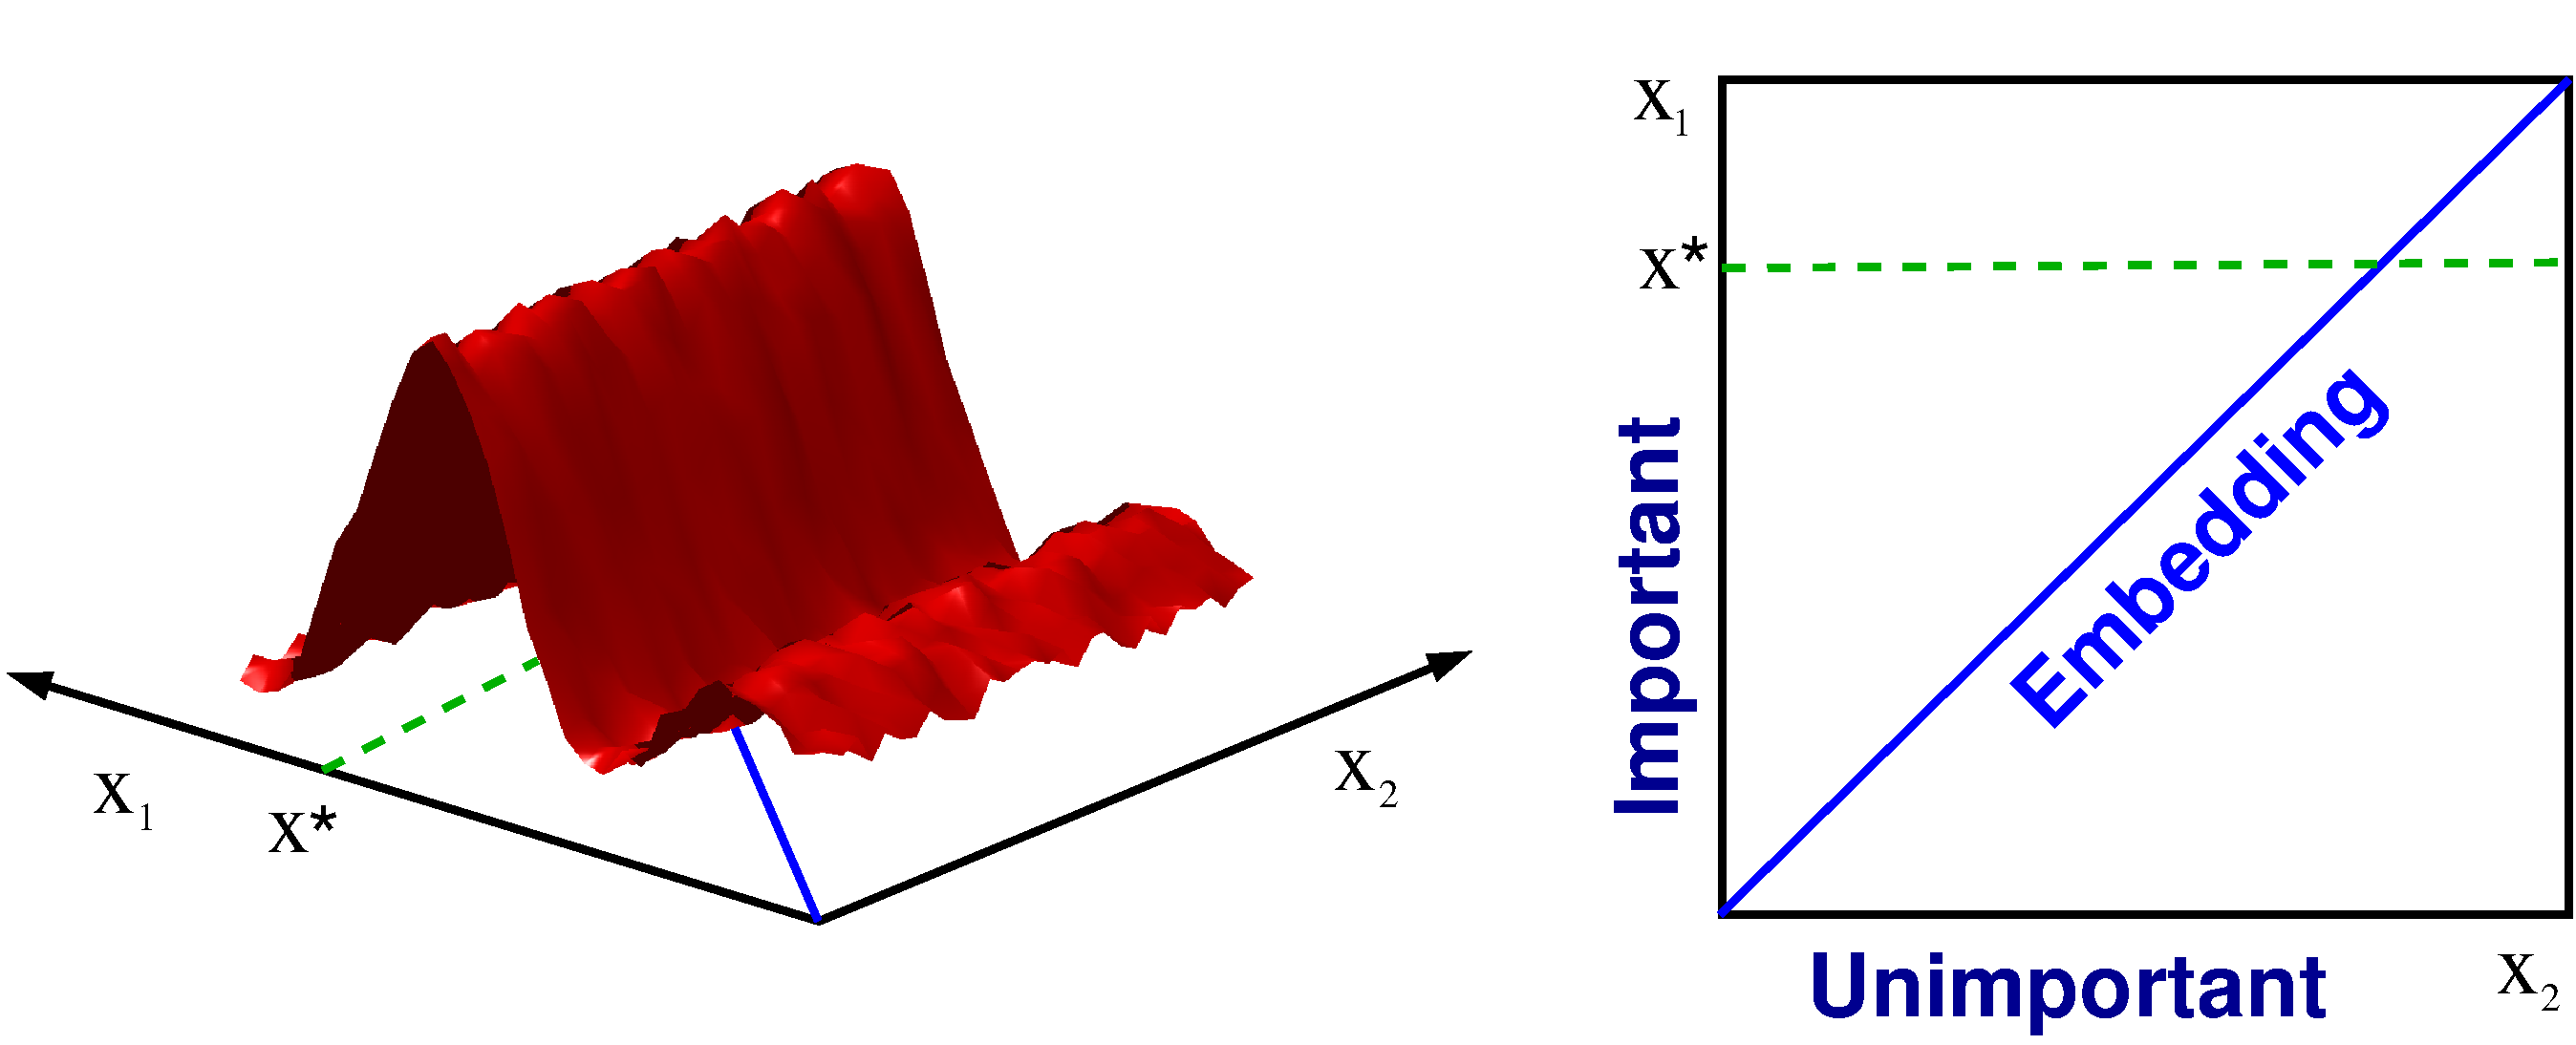
\includegraphics[scale=0.16]{figures/2to1embedding.pdf}
  \centering
  \caption{This function in D=2 dimesions only has d=1 \emph{effective dimension}: the vertical axis indicated with the word important on the right hand side figure. Hence, the $1$-dimensional embedding includes the $2$-dimensional function's optimizer. It is more efficient to search for the optimum along the 1-dimensional random embedding than in the original 2-dimensional space.}
  \label{fig:simple_embedding}
  \vspace*{-4mm}
\end{figure}

Figure \ref{fig:simple_embedding} illustrates our approach in a nutshell.
Assume we know that a given $D=2$ dimensional black-box function $f(x_1, x_2)$ only has $d=1$ important dimensions, but we do not know which of the two dimensions is the important one.
We can then perform optimization in the embedded 1-dimensional subspace defined by $x_1=x_2$ since this is guaranteed to include the optimum. 
This idea enables us to perform Bayesian optimization in a low-dimensional space to
optimize a high-dimensional function with low intrinsic dimensionality. 
Importantly, it is not restricted to cases with axis-aligned intrinsic dimensions.
%
%Following an explanation of GP-based Bayesian optimization (Section \ref{sec:bo}), we introduce the Random EMbedding Bayesian optimization (REMBO) algorithm. Our experiments (Section \ref{sec:experiments}) show that REMBO can solve problems of previously untenable high extrinsic dimensions. They also show that REMBO can achieve state-of-the-art performance when automatically tuning the 47 discrete parameters of a popular linear programming solver. 
%






\section{Bayesian Optimization}\label{sec:bo}

Bayesian optimization has two ingredients that need to be specified: The prior and the acquisition function. In this work, we adopt GP priors. We review GPs very briefly and refer the interested reader to \cite{Rasmussen:2006}.
A GP is a distribution over functions specified by its mean function $m(\cdot)$ and covariance $k(\cdot,\cdot)$. More specifically, given a set of points $\vx_{1:t}$, with $\vx_i \subseteq \mathbb{R}^D$, we have 
$$
\vf(\vx_{1:t}) \sim \mathcal{N}(\vm(\vx_{1:t}), \vK(\vx_{1:t}, \vx_{1:t})),
$$
where $\vK(\vx_{1:t}, \vx_{1:t})_{i,j} = k(\vx_i, \vx_j)$
serves as the covariance matrix. A common choice of $k$ is the squared exponential function,
but many other choices are possible depending on our degree of belief about the smoothness of the objective function.
%Note that $k(x, y) = 1$ when $x = y$ and as $\|x-y\|_2$ increases $k(x, y)$ decreases. This means that two points that are close %by have a bigger covariance and points that are far away from each other have smaller covariance. 

An advantage of using GPs lies in their analytical tractability. In particular, given observations $\vx_{1:n}$ with corresponding values $\vf_{1:t}$, where $f_i = f(\vx_i)$,  and a new point $\vx^{*}$, the joint distribution is given by:
$$
\begin{bmatrix}\vf_{1:t} \\
f^* \end{bmatrix} \sim \mathcal{N}\left( \vm(\vx_{1:t}),  \begin{bmatrix}
\vK(\vx_{1:t}, \vx_{1:t}) & \vk(\vx_{1:t}, \vx^*)\\
\vk(\vx^*, \vx_{1:t}) & k(\vx^*, \vx^*)\end{bmatrix}\right).
$$
For simplicity, we assume that $\vm(\vx_{1:t}) = \mathbf{0}$. Using the Sherman-Morrison-Woodbury formula, one can easily arrive at the posterior predictive distribution:
$$
f^* | \data_t, \vx^* \sim \mathcal{N}(\mu(\vx^*|\data_t), \sigma(\vx^*|\data_t)),
$$
with data $\data_t = \{\vx_{1:t}, \vf_{1:t} \}$, mean
$\mu(\vx^*|\data_t) = \vk(\vx^*, \vx_{1:t}) \vK(\vx_{1:t}, \vx_{1:t})^{-1} \vf_{1:t}$ and variance $\sigma(\vx^*|\data_t) = k(\vx^*, \vx^*)-\vk(\vx^*, \vx_{1:t}) \vK(\vx_{1:t},\vx_{1:t})^{-1} \vk(\vx_{1:t}, \vx^*)$.
That is, we can compute the posterior predictive mean $\mu(\cdot)$ and variance $\sigma(\cdot)$ exactly for any point $\vx^*$.

At each iteration of Bayesian optimization, one has to re-compute the predictive mean and variance. These two quantities are used to construct the second ingredient of Bayesian optimization: The acquisition function. In this work, we report results for the expected improvement acquisition function $u(\vx|\mathcal{D}_t)=\mathbb{E}(\max\{0,f_{t+1}(\vx) - f(\xbest)\} |\data_t)$
\cite{Mockus:1982,Bull:2011}. In this definition, $\xbest = \argmax_{\vx \in \{\vx_{1:t} \} }f(\vx)$
is the element with the best objective value in the first $t$ steps of the optimization process. The next query is:
$\vx_{t+1} = \argmax_{\vx \in {\cal X}} u(\vx|\mathcal{D}_t).$ 
Note that this utility favors the selection of points with high variance (points in regions not well explored) and points with high mean value (points worth exploiting). We also experimented with the UCB acquisition function \cite{Srinivas:2010,deFreitas:2012} and found it to yield similar results. The optimization of the closed-form acquisition function can be carried out by off-the-shelf numerical optimization procedures.
The Bayesian optimization procedure is shown in Algorithm~\ref{alg:bo}. 
\begin{algorithm}
\caption{Bayesian Optimization}
\label{alg:bo}
\begin{algorithmic}[1]
{
\FOR{$t=1,2,\dots$}
  \STATE Find $\vx_{t+1} \in \mathbb{R}^D$ by optimizing the acquisition function $u$: $\vx_{t+1} = \argmax_{\vx \in {\cal X}} u(\vx|\mathcal{D}_t).$ 
  \STATE Augment the data $\mathcal{D}_{t+1} = \{\mathcal{D}_{t}, (\vx_{t+1}, f(\vx_{t+1})) \}$
\ENDFOR
}
\end{algorithmic}
\end{algorithm}















\section{REMBO}\label{sec:rembo}
Before introducing our new algorithm and its theoretical properties, we need to define what we mean by effective dimensionality formally.
\begin{mydefinition}\label{def:effdim}
A function $f: \mathbb{R}^{D} \rightarrow \mathbb{R}$ is said to have \textbf{effective dimensionality} $d_e$, with $d_e < D$, if there exists a linear subspace ${\cal T}$ of dimension $d_e$ such that for all $\vx_{\top} \in {\cal T} \subset \mathbb{R}^D$ and $\vx_{\bot} \in {\cal T}^{\bot} \subset \mathbb{R}^D$, we have $f(\vx) = f(\vx_{\top} + \vx_{\bot}) = f(\vx_{\top})$, where ${\cal T}^{\bot}$ denotes the orthogonal complement of ${\cal T}$. We call ${\cal T}$ the \textbf{effective subspace} of $f$ and ${\cal T}^{\bot}$ the \textbf{constant subspace}.
\end{mydefinition}
This definition simply states that the function does not change along the coordinates $\vx_{\bot}$, and this is why we refer
to ${\cal T}^{\bot}$ as the {constant subspace}.
Given this definition,
the following theorem shows that problems of low effective dimensionality can be solved via random embedding.

\begin{theorem}
\label{prop:1}
Assume we are given a function $f: \mathbb{R}^{D} \rightarrow \mathbb{R}$ with effective dimensionality $d_e$ and a random matrix $\vA \in \mathbb{R}^{D\times d}$ with independent entries sampled according to $\mathcal{N}(0, 1)$ and $d\geq d_e$. Then, with probability 1, for any $\vx \in \mathbb{R}^D$, there exists a $ \vy \in \mathbb{R}^d$ such that $f(\vx) = f(\vA\vy)$.
\end{theorem}
\begin{proof}
Since $f$ has effective dimensionality $d_e$, there exists an effective subspace ${\cal T} \subset \mathbb{R}^D$, such that rank$({\cal T}) = d_e$. Furthermore, any $\vx \in \mathbb{R}^D$ decomposes as
 $\vx = \vx_{\top} + \vx_{\bot}$, where $\vx_{\top} \in {\cal T}$ and $\vx_{\bot} \in {\cal T}^{\bot}$. Hence, $f(\vx) = f(\vx_{\top} + \vx_{\bot}) = f(\vx_{\top}).$ Therefore, without loss of generality, it will suffice to show that for all $\vx_{\top} \in {\cal T}$, there exists a $\vy\in \mathbb{R}^d$ such that $f(\vx_{\top}) = f(\vA\vy)$.

Let $\vPhi \in \mathbb{R}^{D \times d_e}$ be a matrix, whose columns form an orthonormal basis for ${\cal T}$. Hence, for each $\vx_{\top} \in {\cal T}$, there exists a $\vc \in \mathbb{R}^{d_e}$ such that $\vx_{\top} = \vPhi \vc$. Let us for now assume that $\vPhi^{T}\vA$ has rank $d_e$. If $\vPhi^{T}\vA$ has rank $d_e$, there exists a $\vy$ such that $(\vPhi^{T}\vA)\vy=\vc$. The orthogonal projection of $\vA\vy$ onto ${\cal T}$ is given by 
$\vPhi \vPhi^T \vA \vy = \vPhi \vc = \vx_{\top}$.
Thus $\vA\vy = \vx_{\top} + \vx'$ for some $\vx' \in {\cal T}^{\bot}$ since $\vx_{\top}$ is the projection $\vA\vy$ onto ${\cal T}$.
Consequently, $f(\vA\vy) = f(\vx_{\top} + \vx') = f(\vx_{\top})$. 

It remains to show that, with probability one, the matrix $\vPhi^T \vA$ has rank $d_e$.
Let $\vA_{e} \in \mathbb{R}^{D\times d_e}$ be a submatrix of $\vA$ consisting of any $d_e$ columns of $\vA$, which are \emph{i.i.d.} samples distributed according to $\mathcal{N}(\mathbf{0}, \vI)$. Then, $\vPhi^T \va_{i}$ are \emph{i.i.d.} samples from $\mathcal{N}(\mathbf{0}, \vPhi^T \vPhi) = \mathcal{N}(\mathbf{0}_{d_e}, \vI_{d_e\times d_e})$, and so we have $\vPhi^T\vA_e$, when considered as an element of $\mathbb{R}^{d_e^2}$, is a sample from $\mathcal{N}(\mathbf{0}_{d_e^2}, \vI_{d_e^2\times d_e^2})$. On the other hand, the set of singular matrices in $\mathbb{R}^{d_e^2}$ has Lebesgue measure zero, since it is the zero set of a polynomial (i.e. the determinant function) and polynomial functions are Lebesgue measurable. Moreover, the Normal distribution is absolutely continuous with respect to the Lebesgue measure, so our matrix $\vPhi^T \vA_e$ is almost surely non-singular, which means that it has rank $d_e$ and so the same is true of $\vPhi^T \vA$, whose columns contain the columns of $\vPhi^T \vA_e$.
\end{proof}

Theorem~\ref{prop:1} says that given any $\vx \in \mathbb{R}^D$ and a random matrix $\vA \in \mathbb{R}^{D\times d}$, with probability $1$, there is a point $\vy \in \mathbb{R}^d$ such that $f(\vx) = f(\vA\vy)$. 
This implies that for any optimizer $\vx^{\star} \in \mathbb{R}^D$, there is a point $\vy^{\star} \in \mathbb{R}^d$ with $f(\vx^\star) = f(\vA\vy^{\star})$. Therefore, instead of optimizing in the high dimensional space, we can optimize the function $g(\vy) = f(\vA\vy)$ in the lower dimensional space.
This observation gives rise to our new algorithm Bayesian Optimization with Random Embedding (REMBO), described in Algorithm \ref{alg:embed}. REMBO first draws a random embedding (given by $\vA$) and then performs Bayesian optimization in this embedded space.
% computes a bounded region $\mathcal{Y}$ in the low-dimensional space, and 

\begin{algorithm}[h!]
\caption{REMBO: Bayesian Optimization with Random Embedding}
\label{alg:embed}
\begin{algorithmic}[1]
{
\STATE Generate a random matrix $\vA$
\STATE Choose the set $\mathcal{Y}$
\FOR{$t=1,2,\dots$}
  \STATE Find $\vy_{t+1} \in \mathbb{R}^d$ by optimizing the acquisition function $u$: $\vy_{t+1} = \argmax_{\vy\in \mathcal{Y}} u(\vy|\mathcal{D}_t).$ 
  \STATE Augment the data $\mathcal{D}_{t+1} = \{\mathcal{D}_{t}, (\vy_{t+1}, f(\vA\vy_{t+1}) \}$
\STATE Update the kernel hyper-parameters.
\ENDFOR
}
\end{algorithmic}
\end{algorithm}


\begin{figure}[t!]
\centering
  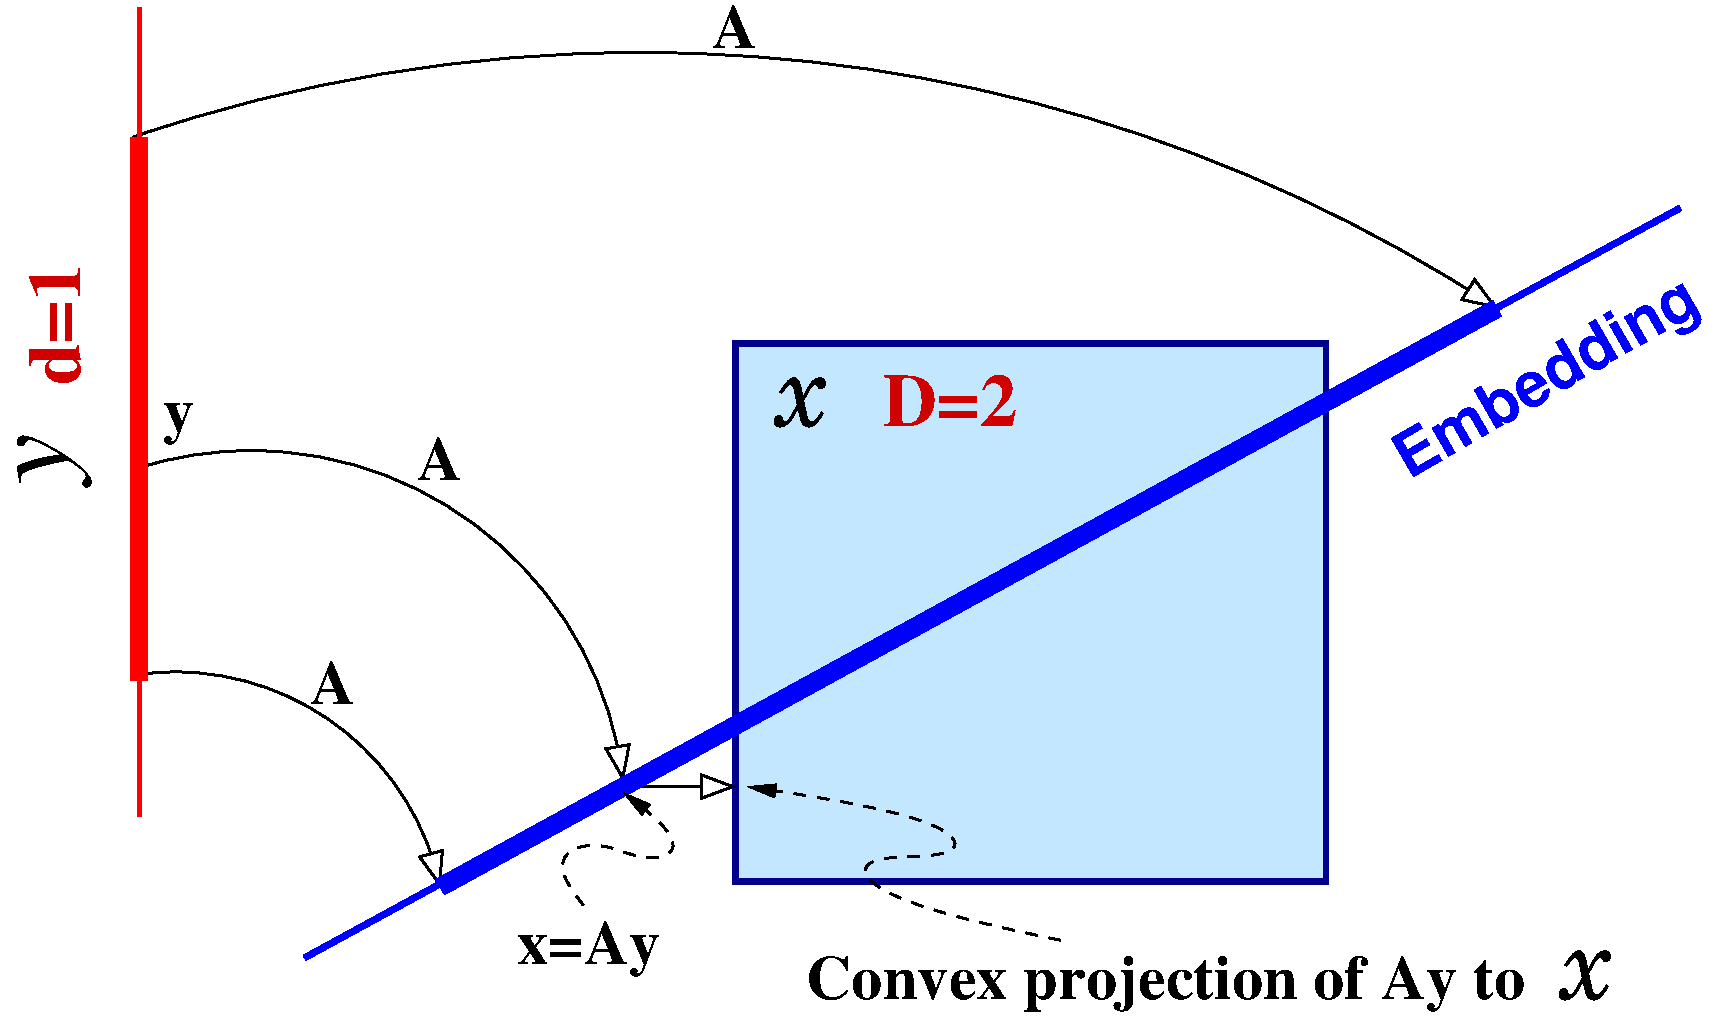
\includegraphics[scale=0.28]{figures/projection.pdf}
  \caption{Embedding from $d=1$ into $D=2$. The box illustrates the 2D constrained space ${\cal X}$, while the thicker red line illustrates the 1D constrained space $\mathcal{Y}$. Note that if $\vA\vy$ is outside $\mathcal{X}$, it is projected onto $\mathcal{X}$. The set $\mathcal{Y}$ must be chosen large enough so that the projection of its image, $\vA \mathcal{Y}$, onto the effective subspace (vertical axis in this diagram) covers the vertical side of the box.}
  \label{fig:proj}
  \vspace{-1em}
\end{figure}

An important detail is how REMBO chooses the bounded region $\mathcal{Y}$, inside which it performs Bayesian optimization. This is important because its effectiveness depends on the size of $\mathcal{Y}$. Locating the optimum within $\mathcal{Y}$ is easier if $\mathcal{Y}$ is small, but if we set $\mathcal{Y}$ too small it may not actually contain the global optimizer (see Figure~\ref{fig:proj}).
In the following theorem, we show that we can choose $\mathcal{Y}$ in a way that only depends on the effective dimensionality $d_e$ such that the optimizer of the original problem is contained in the low-dimensional space with constant probability.
(If $\vA\vy$ is outside the box $\mathcal{X}$, it is projected onto $\mathcal{X}$.)
\begin{theorem}
\label{prop:2}
Suppose we want to optimize a function $f: \mathbb{R}^{D} \rightarrow \mathbb{R}$ with effective dimension $d_e \leq d$ subject to the box constraint $\mathcal{X} \subset \mathbb{R}^D$, where $\mathcal{X}$ is centered around $\mathbf{0}$. Let us denote one of the optimizers by $\vx^{\star}$.
Suppose further that the effective subspace $\cal T$ of $f$ is such that $\cal T$ is the span of $d_e$ basis vectors. 
Let $\vx^{\star}_\top \in \cal{T} \cap \mathcal{X}$ be an optimizer of $f$ inside $\mathcal{T}$. 
If $\vA$ is a $D\times d$ random matrix with independent standard Gaussian entries,
there exists an optimizer $\vy^\star \in \mathbb{R}^{d}$ such that $f(\vA\vy^\star) = f(\vx^\star_\top)$ and $\|\vy^\star\|_2 \leq \frac{\sqrt{d_e}}{\epsilon}\|\vx^{\star}_\top\|_2$ with probability at least $1-\epsilon$.
\end{theorem}
\begin{proof}
Since $\mathcal{X}$ is a box constraint, by projecting $\vx^\star$ to $\cal T$ we get $\vx^\star_\top \in \mathcal{T} \cap \mathcal{X}$. Also, since $\vx^\star =  \vx^\star_\top + \vx_\bot$ for some $\vx_\bot \in \cal T^{\bot}$, we have $f(\vx^\star) = f(\vx^\star_\top)$. Hence, $\vx^\star_\top$ is an optimizer.
By using the same argument as appeared in Theorem~\ref{prop:1}, it is easy to see that with probability $1$ $\forall \vx \in \cal T$ $\exists \vy \in \mathbb{R}^d$ such that $\vA\vy = \vx + \vx_\bot$ where $\vx_\bot \in \cal T^{\bot}$. Let $\vPhi$ be the matrix whose columns form a standard basis for $\cal T$. Without loss of generality, we can assume that 
%\[ \vPhi = \begin{bmatrix}\vI_{d_e} \\
%\mathbf{0} \end{bmatrix} \]
$\vPhi = [\vI_{d_e} \; \mathbf{0} ]^T$.
Then, as shown in Proposition~\ref{prop:1}, there exists a $\vy^\star \in \mathbb{R}^d$ such that $\vPhi \vPhi^{T}\vA \vy^\star = \vx^\star_\top$. Note that for each column of $\vA$, we have
\[ \vPhi \vPhi^{T}\va_i \sim \mathcal{N}\left(\mathbf{0}, \begin{bmatrix}
\vI_{d_e} & {\bf 0}\\
{\bf 0} & {\bf 0}\end{bmatrix}\right). \]
Therefore $\vPhi \vPhi^{T}\vA\vy^\star = \vx^\star_\top$ is equivalent to $\vB\vy^\star = \bar{\vx}^\star_\top$ where $\vB\in \mathbb{R}^{d_e \times d_e}$ is a random matrix with independent standard Gaussian entries and $\bar{\vx}^\star_\top$ is the vector that contains the first $d_e$ entries of $\vx^\star_\top$ (the rest are $0$'s). By Theorem 3.4 of \cite{Sankar:2003}, we have
\[ \mathbb{P}\left[\|\vB^{-1}\|_2 \geq \frac{\sqrt{d_e}}{\epsilon}\right]  \leq \epsilon. \]

Thus, with probability at least $1-\epsilon$, $\|\vy^\star\| \leq \|\vB^{-1}\|_2  \|\bar{\vx}^\star_\top\|_2 = \|\vB^{-1}\|_2  \|\vx^\star_\top\|_2 \leq \frac{\sqrt{d_e}}{\epsilon} \|\vx^\star_\top\|_2$. 
\end{proof}

Theorem~\ref{prop:2} says that if the set $\mathcal{X}$ in the original space is a box constraint, then there exists an optimizer $\vx^\star_\top \in \mathcal{X}$ that is $d_e$-sparse such that with probability at least $1-\epsilon$, $\|\vy^\star\|_2 \leq \frac{\sqrt{d_e}}{\epsilon}\|\vx^{\star}_\top\|_2$ where $f(\vA\vy^\star) = f(\vx^\star_\top)$. If the box constraint is $\mathcal{X} = [-1,1]^D$ (which is always achievable through rescaling), we have with probability at least $1-\epsilon$ that 
\[ \|\vy^\star\|_2 \leq \frac{\sqrt{d_e}}{\epsilon}\|\vx^{\star}_\top\|_2 \leq \frac{\sqrt{d_e}}{\epsilon}\sqrt{d_e}. \]
%\note{FH: fixed a typo. It said: $\|\vy^\star\|_2 \leq \frac{\sqrt{d}}{\epsilon}\|\vx^{\star}_\bot\|_2 \leq \frac{\sqrt{d}}{\epsilon}\sqrt{d}.$}
Hence, to choose $\mathcal{Y}$, we just have to make sure that the ball of radius $d_e/\epsilon$ satisfies $({\bf 0}, \frac{d_e}{\epsilon} ) \subseteq \mathcal{Y}$. In most practical scenarios, we found that the optimizer does not fall on the boundary which implies that $\|\vx^{\star}_\top\|_2 < d_e$. Thus setting $\mathcal{Y}$ too big may be unnecessarily wasteful. In all our experiments we set $\mathcal{Y}$ to be $[-\sqrt{d}, \sqrt{d}]^d$.

%\subsection{Increasing the Success Rate of REMBO}\label{sec:increasing_rembo_success}

Theorem~\ref{prop:2} only guarantees that $\mathcal{Y}$ contains the optimum with probability at least $1-\epsilon$;
with probability $\delta \le \epsilon$ the optimizer lies outside of $\mathcal{Y}$. There are several ways to guard against this problem. One is to simply run REMBO multiple times with different independently drawn random embeddings. 
%
Since the probability of failure with each embedding is $\delta$, 
the probability of the optimizer not being included in the considered space of $k$ independently drawn embeddings is $\delta^k$. 
Thus, the failure probability vanishes exponentially quickly in the number of REMBO runs, $k$. 
Note also that these independent runs can be trivially parallelized to harness the power of
modern multi-core machines and large compute clusters.
%
%Another way of increasing REMBO's success rate is to increase the dimensionality $d$ it uses internally. When $d > d_e$, with probability $1$ we have ${ d \choose d_e }$ different embeddings of dimensionality $d_e$. 
%That is,
%we only need to select $d_e$ columns of $\vA \in \mathbb{R}^{D \times d}$ to represent the $d_e$ relevant dimensions of $\vx$.
%We can do this by choosing $d_e$ sub-components of the $d$-dimensional vector $\vy$ while setting the remaining components to zero. 
%Informally, since we have more embeddings, it is more likely that one of these will include the optimizer.
%In our experiments, we will assess the merits and shortcomings of these two strategies. 

\subsection{Choice of Kernel}\label{sec:choice_of_kernel}

We begin our discussion on kernels with the definition of the squared exponential kernel between two points, $\vy^{(1)}, \vy^{(2)}$, on ${\cal Y} \subseteq \mathbb{R}^d$.
Given a length scale $r > 0$, we define the corresponding {squared exponential} kernel as 
\[ k_{\ell}^d(\vy^{(1)},\vy^{(2)}) = \exp\left({-\frac{\|\vy^{(1)}-\vy^{(2)}\|^2}{2\ell^2}}\right). \]
It is possible to work with two variants of this kernel. 
First, we can use $k_{\ell}^d(\vy^1, \vy^2)$ as above. We refer to this kernel as the low-dimensional kernel. We can also adopt an implicitly defined high-dimensional kernel on 
$\mathcal{X}$:
$$k_{\ell}^D(\vy^{(1)}, \vy^2) = \exp\left( -\frac{\| p_{\mathcal{X}}(\vA\vy^{(1)}) - p_{\mathcal{X}}(\vA\vy^{(2)}) \|^2}{2\ell^2} \right),$$
where $p_{\mathcal{X}}:\mathbb{R}^D \rightarrow \mathbb{R}^D$ is the standard projection operator for our box-constraint: $p_{\mathcal{X}}(\vy) = {\arg \min}_{\vz\in \mathcal{X}} \|\vz-\vy\|_2$; see Figure~\ref{fig:proj}. 


Note that when using the high-dimensional kernel, we are fitting the GP in $D$ dimensions. However, the search space is no longer the box $\mathcal{X}$, but it is instead given by the much smaller subspace $\{p_{\mathcal{X}}(\vA\vy): \vy \in {\cal Y} \}$. \emph{Importantly, in practice it is easier to maximize the acquisition function in this subspace.} Our experiment on automatic algorithm configuration will show that indeed optimizing the acquisition function in low dimensions leads to significant gains of REMBO over standard Bayesian optimization.


%Both kernel choices have strengths and weaknesses. For the low-dimensional kernel, exploring in the region of the embedding outside of ${\cal X}$ (see Figure 2) may be wasteful because two points far apart in this region may be projected via $p_{\mathcal{X}}$ to nearby points on the boundary of ${\cal X}$. The high-dimensional kernel is not affected by this problem because the search is conducted directly on 
% $\{p_{\mathcal{X}}(\vA\vy): \vy \in {\cal Y} \}$. However, t
% 
 
The low-dimensional kernel has the benefit of only having to construct a GP in the space of intrinsic dimensionality $d$, whereas the high-dimensional kernel has to construct the GP in a space of extrinsic dimensionality $D$. However,
the choice of kernel also depends on whether our variables are continuous, integer or categorical. The categorical case is important because we often encounter optimization problems that contain discrete choices.
% (in fact, we focus on this case in our application in the experiments). %FH: repetitive & thus commented out for space.
We define our kernel for categorical variables as:
$$k^D_{\lambda}(\vy^{(1)}, \vy^{(2)}) = \exp\left(-\frac{\lambda}{2} g(s(\vA\vy^{(1)}), s(\vA\vy^{(2)}))^2\right),$$
where $\vy^{(1)}, \vy^{(2)} \in {\cal Y} \subset \mathbb{R}^d$ and $g$ defines the distance between 2 vectors. The function $s$ maps continuous vectors to discrete vectors. In more detail, $s(\vx)$ first projects $\vx$ to $[-1,1]^D$ to generate $\bar{\vx}$. For each dimension $\bar{x}_i$ of $\bar{\vx}$, $s$ then maps $\bar{x}_i$ to the corresponding discrete parameters by scaling and rounding. In our experiments, following~\cite{Hutter:2009}, we defined $g(\vx^{(1)}, \vx^{(2)}) = |\{i: x^{(1)}_i \neq x^{(2)}_i\}|$ 
so as not to impose an artificial ordering between the values of categorical parameters. 
In essence, we measure the distance between two points in the low-dimensional space as the distance between their mappings in the high-dimensional space. 

Our demonstration of REMBO, in the domain of algorithm configuration, will use the high-dimensional kernel because the parameters in need of tuning are categorical. However, to provide the reader with a taste of the potential gains that the low-dimensional kernel could offer in continuous spaces, we will use a synthetic optimization problem. This synthetic example will also allow us to easily discuss different properties of the algorithm, including rotational invariance and dependency on $d$.

Finally, when using the high-dimensional kernel, the regret bounds of \cite{Srinivas:2010,Bull:2011,deFreitas:2012} apply. For the low-dimensional case, we have derived regret bounds that only depend on the intrinsic dimensionality. For lack of space, these are covered in a longer technical report version of this paper~\cite{WanEtAl13:REMBO_arXiv}.
%will present these in a longer technical report version of this paper.






\begin{figure*}[t!]
  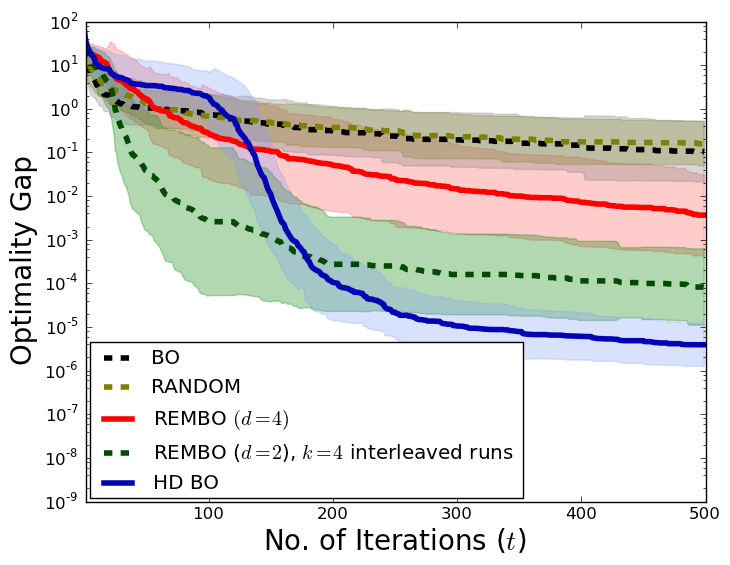
\includegraphics[scale=0.4]{figures/branin_dis_25.png}
  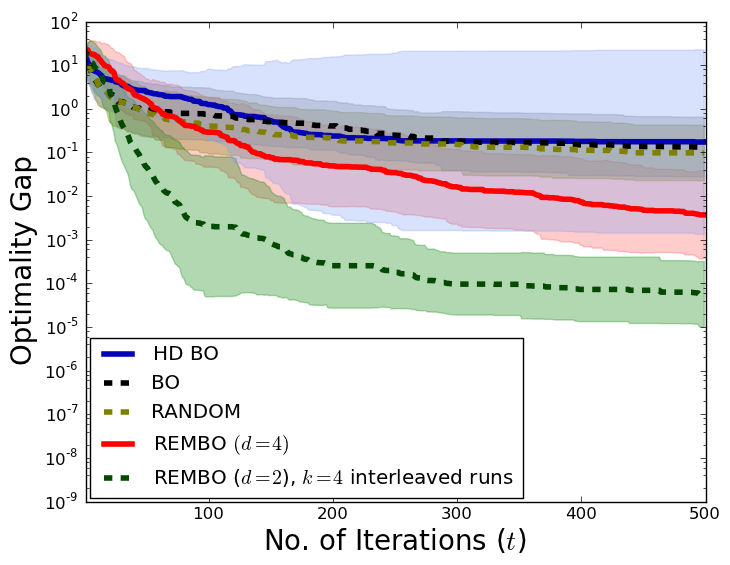
\includegraphics[scale=0.4]{figures/branin_dis_rot.png}
  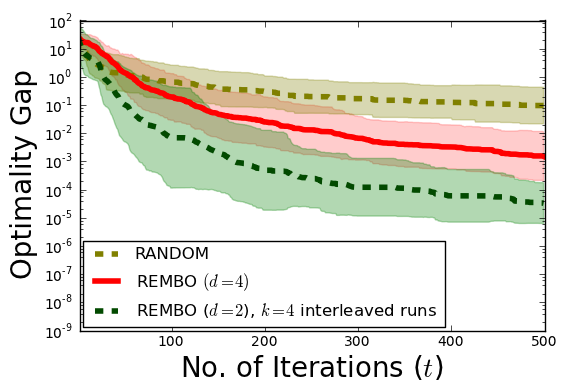
\includegraphics[scale=0.4]{figures/branin_dis_1b.png}
  \caption{Comparison of random search (RANDOM), Bayesian optimization (BO),
  method by~\protect\cite{Chen:2012} (HD BO), and REMBO.
Left: $D=25$ extrinsic dimensions; Middle: $D=25$, with a rotated objective function; Right: $D=10^9$ extrinsic dimensions. We plot means and $1/4$ standard deviation confidence intervals of the optimality gap across 50 trials.}
  \label{fig:standard}
  \vspace{-1.0em}
\end{figure*}





\section{Experiments}\label{sec:experiments}


%
%To illustrate the performance of REMBO with the low dimensional kernel, we adopt simple
%synthetic functions of small intrinsic dimensionality $d_e=2$ but 
%extrinsic dimension $D$ up to $1$ billion. This demonstrates REMBO's independence of $D$. The synthetic experiment also enables us to study the choice of $d$ and shows that REMBO is indeed rotationally invariance.
%To illustrate the performance of REMBO with the high dimensional kernel, 
%we apply REMBO to automatically optimize the 47 parameters of a widely-used linear programming solver and demonstrate that it achieves state-of-the-art performance.

For all our experiments, we used a single robust version of REMBO that automatically sets its GP's length scale parameter using a variant of maximum likelihood (see the technical report \cite{WanEtAl13:REMBO_arXiv} for details).
For each optimization of the acquisition function, this version runs both DIRECT \cite{Jones:1993} and CMA-ES~\cite{Hansen:2001:CDS:1108839.1108843} and uses the result of the better of the two.
Source code for REMBO, as well as all data used in our experiments is publicly available at \url{https://github.com/ziyuw/rembo}.
% \note{FH: We promised in the submission ``Source code for REMBO, as well as all data used in our experiments, will be made publicly available after the double-blind review.'' Now we need to do it, so I'm pointing to a new github directory.}

%Some of our experiments required substantial computational resources, with the computational 
%expense of each experiment depending mostly on the cost of evaluating the respective blackbox function. 
%While the synthetic experiments in Section \ref{exp:billion} only required minutes for each run of each method, optimizing the mixed integer programming solver in Section \ref{exp:mip_opt} required 4-5 hours per run.
%
%In each experiment, we study the effect of the two methods for increasing REMBO's success rate introduced in Section \ref{sec:increasing_rembo_success} by running different numbers of independent REMBO runs with different settings of its internal dimensionality $d$.





\subsection{Bayesian Optimization in a Billion Dimensions}\label{exp:billion}

%In this section, we study REMBO's invariance properties using synthetic data, empirically evaluate strategies for increasing its success probability,
%and, most importantly, add empirical evidence to our theoretical finding from Section \ref{sec:rembo} that REMBO's performance is independent of the extrinsic dimensionality $D$
%when using the low-dimensional kernel $k_{\ell}^d(\vy^1, \vy^2)$.
%We show that when using that kernel, REMBO has no problem scaling up to as many as $1$ billion dimensions.


The experiments in this section employ a standard $d_e=2$-dimensional benchmark function for Bayesian optimization, embedded in a $D$-dimensional space. That is, we add $D-2$ additional dimensions which do not affect the function at all.
More precisely, the function whose optimum we seek is $f(\vx_{1:D}) = g(x_i,x_j)$, where $g$ is the Branin function
(for its exact formula, see \cite{Lizotte:2008}) and where $i$ and $j$ are selected once using a random permutation.
To measure the performance of each optimization method, we used the \emph{optimality gap}: the difference of the best function value it found and the optimal function value.   

\begin{table}[h]
\scriptsize
\begin{center}
\begin{tabular}{ l |  c  c  c}
\hline
$k$ & $d=2$ & $d=4$ & $d=6$ \\
\hline
  10& 0.0022 $\pm$ 0.0035 & 0.1553 $\pm$ 0.1601 & 0.4865 $\pm$  0.4769 \\
  5 & 0.0004 $\pm$ 0.0011 & 0.0908 $\pm$ 0.1252 & 0.2586 $\pm$ 0.3702 \\
  4 & 0.0001 $\pm$ 0.0003 & 0.0654 $\pm$ 0.0877 & 0.3379 $\pm$ 0.3170 \\
  2 & 0.1514 $\pm$ 0.9154 & 0.0309 $\pm$ 0.0687 & 0.1643 $\pm$ 0.1877 \\
  1 & 0.7406 $\pm$ 1.8996 & 0.0143 $\pm$ 0.0406 & 0.1137 $\pm$ 0.1202 \\
\end{tabular}
\end{center}
\vspace*{-3mm}
\caption{Optimality gap for $d_e=2$-dimensional Branin function embedded in $D=25$ dimensions, for
REMBO variants using a total of $500$ function evaluations. The variants differed in the internal dimensionality $d$ and in the number of interleaved runs $k$ (each such run was only allowed $500/k$ function evaluations).
%We initialized all methods to the same random point and 
We show mean and standard deviations of the optimality gap achieved after 500 function evaluations. 
\label{tab:rembo_variants_results}}
\vspace*{-3mm}
\end{table}

We evaluate REMBO using a fixed budget of $500$ function
evaluations that is spread across multiple interleaved runs ---
for example, when using $k = 4$ interleaved REMBO runs,
each of them was only allowed $125$ function evaluations. 
We study the choices of $k$ and $d$ by considering several combinations of these values.
The results in Table \ref{tab:rembo_variants_results} demonstrate that interleaved runs helped improve REMBO's performance.
We note that in 13/50 REMBO runs, the global optimum was indeed not contained in the box $\mathcal{Y}$ REMBO searched with $d=2$; this is the reason for the poor mean performance of REMBO with $d=2$ and $k=1$.
However, the remaining $37$ runs performed very well, and REMBO thus performed well when using multiple interleaved runs: with a failure rate of 13/50=0.26 per independent run, the failure rate using $k=4$ interleaved runs is only $0.26^4\approx 0.005$. One could easily achieve an arbitrarily small failure rate by using many independent parallel runs. 
Using a larger $d$ is also effective in increasing the probability of the optimizer falling into REMBO's box $\mathcal{Y}$ but at the same time slows down REMBO's convergence (such that interleaving several short runs loses its effectiveness). 
 
Next, we compared REMBO to standard Bayesian optimization (BO) and to random search, for an extrinsic dimensionality of $D=25$. 
Standard BO is well known to perform well in low dimensions, but to degrade above a tipping point of about 15-20 dimensions. Our results for $D=25$ (see Figure \ref{fig:standard}, left) confirm that BO performed rather poorly just above this critical dimensionality (merely tying with random search). 
REMBO, on the other hand, still performed very well in 25 dimensions.

One important advantage of REMBO is that --- in contrast to the approach of \cite{Chen:2012} --- it does not require the effective dimension to be coordinate aligned. To demonstrate this fact empirically, we rotated the embedded Branin function by an orthogonal rotation matrix $\vR \in \mathbb{R}^{D\times D}$. That is, we replaced $f(\vx)$ by $f(\vR \vx)$.
Figure~\ref{fig:standard} (middle) shows that REMBO's performance is not affected by this rotation. 
%
Finally, since REMBO is independent of the extrinsic dimensionality $D$ as long as the intrinsic dimensionality $d_e$ is small, it performed just as well in $D=1\,000\,000\,000$ dimensions (see Figure \ref{fig:standard}, right). 
To the best of our knowledge, the only other existing method that can be run in such high dimensionality is random search.

For reference, we also evaluated the method of \cite{Chen:2012} for these functions, confirming that it does not handle rotation gracefully: 
while it performed best in the non-rotated case for $D=25$, it performed worst in the rotated case (tying with standard BO). It could not be used efficiently for more than $D=1,000$.
%other recent method targetting 
%Experiments with the code of \cite{Chen:2012} (not reported in detail for lack of space) confirm that their method \emph{is} affected by the rotation: while it performed best in the non-rotated case, it performed worst in the rotated case (tying with standard BO).
% it performed just as poorly as standard BO.










%
%
%To compare to the best possible scenario, we do Bayesian optimization directly on the Branin function. Next, to study the effect of extrinsic dimensionality on the proposed approach, we embed the Branin function in a one million dimensional space and run the proposed approach. As discussed in the previous section, we know that the true optimizer does not always fall into the bound $\mathcal{B}$ in the lower dimensional space. To illustrate the efficiency of our method we ensured that at least one optimizer falls into $\mathcal{B}$ by repeatedly drawing $\vA$. Here $\mathcal{B}$ is chosen to be $[0, 1]^d$. 
%
%For the third experiment, we choose our embedding dimension $d$ to be $4$ which is higher than the effective dimension $d_e = 2$. We show that by doing this, the failure probability decreases dramatically. Unlike in the previous experiment, we do not try to ensure that an optimizer falls into $\mathcal{B}$. To further lower the probability of not including an optimizer, we set the bound to be $[0, 1]^d \times \sqrt d$. In doing so we lowered the probability of failure to $0.01$.
%
%The fourth experiment shows that our approach is still valid when the effective dimensions are not coordinate-aligned. The embedded Branin function is rotated by an orthogonal rotation matrix $R \in \mathbb{R}^{D\times D}$. As in the last $2$ experiments, we set $D$ to be one million and ensure that one optimizer falls into $\mathcal{B}$ where $\mathcal{B} = [0, 1]^d$. Finally, we embed the Branin function in a $20$ dimensional space and try Bayesian optimization on this high dimensional space. 
%
%All of the above experiments are repeated $20$ times each with $500$ iterations. Figure \ref{fig:standard}~(left) presents the result by summarizing the mean and $\frac{1}{5}$ of the standard deviation of $G_t$ across different runs. Notice that when an optimizer is contained in $\mathcal{B}$, REMBO is comparable to the BO when $d = 2$ as they both locate the maximum well within $100$ iterations. This is significant as it demonstrates that REMBO is not affected by the extrinsic dimensionality which in this case is one million. 
%In Table 1 we summarize the empirical percentage of times where the true optimizer is contained in $\mathcal{B} = [0, 1]^d$. Although we can not guarantee that the true optimizer is contained in $\mathcal{B}$, we argue that REMBO is still preferable over BO when the dimensionality is high. Observe that BO in $20$ dimensions could not find the maximum within $500$ iterations while by repeating REMBO $5$ times each with $100$ iterations, we can locate the optimizer with failure probability approximately equal to $(1-0.5951)^5 = 0.0109$. Further, we must remember that BO would become infeasible in high dimensions whereas our approach would scale up to arbitrary high dimensions as long as the effective dimensionality is relatively low. Figure \ref{fig:standard}~(left) also shows that despite the fact that we do not check whether the optimizer falls into $\mathcal{B}$ when $d=4$, REMBO still manages to locate the optimum after $400$ iterations. The experimental results show that when $d=4$ and $\mathcal{B} = [0, 
%1]^d \times \sqrt d$, the probability of having at least one optimizer in $\mathcal{B}$ is approximately $0.99$. Whereas the approach of Chen et al \cite{Chen:2012} requires the effective dimension to be coordinate aligned, REMBO does not.  
%
%For the Hartmann3 function, we compared REMBO with BO in the original and high dimensional space. All of the experiments are repeated $20$ times each with $200$ iterations. Figure \ref{fig:standard}~(right) summarizes the result by plotting the mean and $\frac{1}{5}$ of the standard deviation $G_t$. The results on the Hartmann3 confirms the findings from the Branin function. It is interesting to note, however, REMBO in this case converges faster than BO in the original space. We attribute this to our choices of hyper-parameters for the GP.
%
%
%
%
%
%
%
%












\subsection{Automatic Configuration of a Mixed Integer Linear Programming Solver}\label{exp:mip_opt}

\begin{figure}[h!]
\begin{center}
  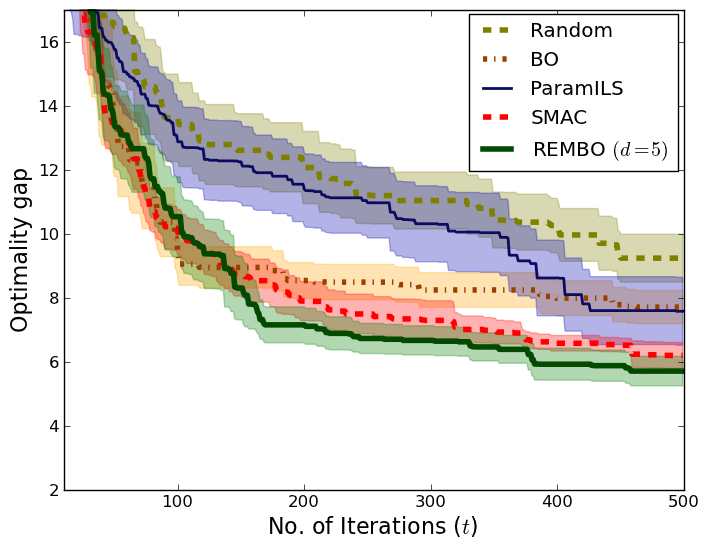
\includegraphics[scale=0.35]{figures/lpsolve.png}\\
  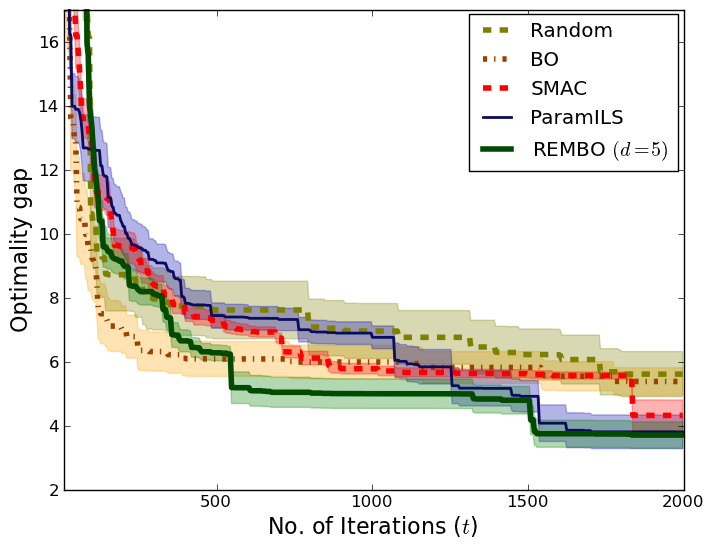
\includegraphics[scale=0.35]{figures/lpsolve_interleave.png}
  \caption{Performance for configuration of \texttt{lpsolve}; we show the optimality gap \texttt{lpsolve} achieved with the configurations found by the various methods (lower is better). Top: a single run of each method; Bottom: performance with $k=4$ interleaved runs. We plot means and $1/4$ standard deviations over 20 repetitions of the experiment.
        %results of 20  confidence. Note that the standard deviation of the mean would be slightly smaller than the ones plotted as we repeat the experiment 20 times.
        }
\label{fig:lpsolve}
\end{center}
\vspace*{-3mm}
\end{figure}

State-of-the-art algorithms for solving hard computational problems tend to parameterize several design choices in order to allow a customization of the algorithm to new problem domains. Automated methods for algorithm configuration have recently demonstrated that substantial performance gains of state-of-the-art algorithms can be achieved in a fully automated fashion~\cite{Mockus:1999,Hutter:2010,ValEtAl11,Bergstra:2011,Wang:2011}. These successes have led to a paradigm shift in algorithm development towards the 
active design of highly parameterized frameworks that can be automatically customized to particular problem domains using optimization~\cite{Hoos:2012:PO:2076450.2076469,Bergstra:model_search}.

%It has long been suspected that the resulting algorithm configuration problems have low dimensionality~\cite{Hutter:2009}. 
It has recently been demonstrated that many algorithm configuration problems have low dimensionality~\cite{Hutter:2013_KeyParameters}. 
Here, we demonstrate that REMBO can exploit this low dimensionality even in the discrete spaces typically encountered in algorithm configuration. 
We use a configuration problem obtained from \cite{Hutter:2010}, aiming to configure the 40 binary and 7 categorical parameters of \texttt{lpsolve}\footnote{http://lpsolve.sourceforge.net/}, a popular mixed integer linear programming solver that has been downloaded over 40\,000 times in the last year.
The objective is to minimize the optimality gap \texttt{lpsolve} can obtain in a time limit of five seconds for a mixed integer programming (MIP) encoding of a wildlife corridor problem from computational sustainability~\cite{ghs08:connection}.
Algorithm configuration aims to improve performance for a representative set of problem instances, and effective methods need to solve two orthogonal problems: searching the parameter space effectively and deciding how many resources to spend in each evaluation (to trade off computational overhead and over-fitting). Our contribution is for the first of these problems; to focus on how effectively the different methods search the parameter space, we only consider configuration on a single problem instance (i.e., a deterministic blackbox optimization problem; further work is required to tackle general algorithm configuration problems with randomized algorithms and distributions of problem instances).

Due to the discrete nature of this optimization problem, we could only apply REMBO using the high-dimensional kernel for categorical variables $k^D_{\lambda}(\vy^{(1)}, \vy^{(2)})$ described in Section \ref{sec:choice_of_kernel}. While we have not proven any theoretical guarantees for discrete optimization problems, REMBO appears to effectively exploit the low effective dimensionality of at least this particular optimization problem.

%Ordinary:
%1,4
%1,5
%3,4
%3,5
%
%Interleaved:
%1,4
%1,5
%3,4
%3,5
%
%SMAC(1), Paramils(2), REMBO(3), Random(4), BO(5). 

Figure \ref{fig:lpsolve} (top) compares BO, REMBO, and the baseline random search against ParamILS (which was used for all configuration experiments in \cite{Hutter:2010})
%ParamILS~\cite{ParamILS-JAIR} (which was used for all configuration experiments in~\cite{Hutter:2010}), 
and SMAC \cite{Hutter:2011}. 
ParamILS and SMAC were specifically designed for the configuration of algorithms with many discrete parameters and define the current state of the art for this problem. Nevertheless, here SMAC and our vanilla REMBO method performed best. Based on a Mann–Whitney U test with Bonferroni multiple-test correction, they both yielded statistically significantly better results than both Random and standard BO; no other performance differences were significant.
The figure only shows REMBO with $d=5$ to avoid clutter, but we did not optimize this parameter; the only other value we tried ($d=3$) resulted in indistinguishable performance. 

As in the synthetic experiment, REMBO's performance could be further improved by using multiple interleaved runs. 
However, it is known that multiple independent runs also benefit the other procedures, especially ParamILS~\cite{HutHooLey12-ParallelAC}. Thus, to be fair, we re-evaluated all approaches using interleaved runs. Figure \ref{fig:lpsolve} (bottom) shows that ParamILS and REMBO benefitted most from interleaving $k=4$ runs. However, the statistical test results did not change, still showing that SMAC and REMBO outperformed Random and BO, with no other significant performance differences.

% \note{FH: Ziyu, we need to add statistical significance here that the reviewer complained about! You gave significance results in the rebuttal, but I don't recall them and I don't recall the test you used, either. Can you please mention this here?}

\section{Conclusion} \label{sec:conclusion}


This paper has shown that it is possible to use random embeddings in Bayesian optimization to optimize functions 
of high extrinsic dimensionality $D$, provided that they have low intrinsic dimensionality $d_e$. 
The new algorithm, REMBO, only requires a simple modification of the original Bayesian optimization algorithm; namely multiplication by a random matrix. 
We confirmed REMBO's independence of $D$ empirically by optimizing low-dimensional functions embedded in high dimensions. 
Finally, we demonstrated that REMBO achieves excellent performance for optimizing the 47 discrete parameters of a popular mixed integer programming solver,
thereby providing further evidence for the observation (already put forward by Bergstra, Hutter and colleagues) that, for many problems of great practical interest, the number of 
important dimensions indeed appears to be much lower than their extrinsic dimensionality. Of course, we do not yet know how many practical optimization problems fall within the class of problems where REMBO applies. With time and the release of the code, we will find more evidence. For the time being, the success achieved in the examples presented in this paper 
%(including the automatic configuration of a very popular solver) %FH: repetitive, so I commented it to save space.
is very encouraging.





%\appendix

%\section{\LaTeX{} and Word Style Files}\label{stylefiles}

%The 


%% The file named.bst is a bibliography style file for BibTeX 0.99c
%\renewcommand{\baselinestretch}{1.05}
\small
\bibliographystyle{named}
\bibliography{bayesopt}

\end{document}